\RequirePackage[l2tabu,orthodox]{nag}

% TODO: decide if one-sided/two-sided
%\documentclass[headsepline,footsepline,footinclude=false,fontsize=11pt,paper=a4,listof=totoc,bibliography=totoc,BCOR=12mm,DIV=12]{scrbook} % two-sided
\documentclass[headsepline,footsepline,footinclude=false,oneside,fontsize=11pt,paper=a4,listof=totoc,bibliography=totoc]{scrbook} % one-sided

% TODO: change citation style in settings
\PassOptionsToPackage{table,svgnames,dvipsnames}{xcolor}

\usepackage[utf8]{inputenc}
\usepackage[T1]{fontenc}
\usepackage[sc]{mathpazo}
\usepackage[ngerman,american]{babel}
\usepackage[autostyle]{csquotes}
\usepackage[%
  backend=biber,
  url=false,
  style=alphabetic,
  maxnames=4,
  minnames=3,
  maxbibnames=99,
  giveninits,
  uniquename=init]{biblatex} % TODO: adapt citation style

% \usepackage{ffcode} % Would be nice to have, but does not work with scrhack
% \usepackage{minted}
% \usemintedstyle{vs}

\usepackage{graphicx}
\usepackage{scrhack} % necessary for listings package
\usepackage{listings}
\usepackage{lstautogobble}
\usepackage{tikz}
\usepackage{pgfplots}
\usepackage{pgfplotstable}
\usepackage{booktabs}
\usepackage[final]{microtype}
\usepackage{caption}
\usepackage[hidelinks]{hyperref} % hidelinks removes colored boxes around references and links
\usepackage{verbatim}
\usepackage{adjustbox}
\usepackage{fancyvrb}

\usepackage{xcolor}
\usepackage{array}
\usepackage{geometry}
\usepackage{placeins}


\newenvironment{myverbatim}{%
 \VerbatimEnvironment
 \begin{adjustbox}{max width=\linewidth}
 \begin{BVerbatim}
  }{
  \end{BVerbatim}
 \end{adjustbox}
}


\bibliography{bibliography}

\setkomafont{disposition}{\normalfont\bfseries} % use serif font for headings
\linespread{1.05} % adjust line spread for mathpazo font

% Add table of contents to PDF bookmarks
\BeforeTOCHead[toc]{{\cleardoublepage\pdfbookmark[0]{\contentsname}{toc}}}

% Define TUM corporate design colors
% Taken from http://portal.mytum.de/corporatedesign/index_print/vorlagen/index_farben
\definecolor{TUMBlue}{HTML}{0065BD}
\definecolor{TUMSecondaryBlue}{HTML}{005293}
\definecolor{TUMSecondaryBlue2}{HTML}{003359}
\definecolor{TUMBlack}{HTML}{000000}
\definecolor{TUMWhite}{HTML}{FFFFFF}
\definecolor{TUMDarkGray}{HTML}{333333}
\definecolor{TUMGray}{HTML}{808080}
\definecolor{TUMLightGray}{HTML}{CCCCC6}
\definecolor{TUMAccentGray}{HTML}{DAD7CB}
\definecolor{TUMAccentOrange}{HTML}{E37222}
\definecolor{TUMAccentGreen}{HTML}{A2AD00}
\definecolor{TUMAccentLightBlue}{HTML}{98C6EA}
\definecolor{TUMAccentBlue}{HTML}{64A0C8}

% Settings for pgfplots
\pgfplotsset{compat=newest}
\pgfplotsset{
  % For available color names, see http://www.latextemplates.com/svgnames-colors
  cycle list={TUMBlue\\TUMAccentOrange\\TUMAccentGreen\\TUMSecondaryBlue2\\TUMDarkGray\\},
}

% Settings for lstlistings
\lstset{%
  basicstyle=\ttfamily,
  columns=fullflexible,
  autogobble,
  keywordstyle=\bfseries\color{TUMBlue},
  stringstyle=\color{TUMAccentGreen}
}


% TODO: change thesis information
\newcommand*{\getUniversity}{Technische Universität München}
\newcommand*{\getFaculty}{TUM School of Computation, Information and Technology}
\newcommand*{\getTitle}{eBPF-Assisted Relays for Multimedia Streaming}
\newcommand*{\getTitleGer}{eBPF-Unterstützung für Multimedia-Streaming-Netzknoten}
\newcommand*{\getAuthor}{Daniel Alexander Antonius Pfeifer}
\newcommand*{\getDoctype}{Bachelor's Thesis in Informatics}
\newcommand*{\getSupervisor}{Prof.~Dr.-Ing. Jörg Ott}
\newcommand*{\getAdvisor}{Mathis Engelbart, M.Sc.}
\newcommand*{\getSubmissionDate}{15.08.2024}
\newcommand*{\getSubmissionLocation}{Munich}


\definecolor{mGreen}{rgb}{0,0.6,0}
\definecolor{mGray}{rgb}{0.5,0.5,0.5}
\definecolor{mPurple}{rgb}{0.58,0,0.82}
\definecolor{backgroundColour}{rgb}{0.95,0.95,0.92}

% Define a custom column type for wrapping text
\newcolumntype{L}[1]{>{\raggedright\arraybackslash}p{#1}}

\lstdefinestyle{CStyle}{
    basicstyle=\ttfamily\small,
    backgroundcolor=\color{white},
    commentstyle=\color{mGreen},
    keywordstyle=\color{magenta}\bfseries,
    numberstyle=\tiny\color{mGray},
    stringstyle=\color{mPurple},
    breakatwhitespace=false,         
    breaklines=true,                 
    captionpos=b,                    
    keepspaces=true,                 
    numbers=left,                    
    numbersep=5pt,                  
    showspaces=false,                
    showstringspaces=false,
    showtabs=false,                  
    tabsize=2,
    frame=single,
    language=C
}

\lstdefinestyle{GoStyle}{
    language=Go,
    basicstyle=\ttfamily\small,
    keywordstyle=\color{blue}\bfseries,
    commentstyle=\color{mGreen},
    stringstyle=\color{red},
    numberstyle=\tiny\color{gray},
    backgroundcolor=\color{white},
    frame=single,
    tabsize=4,
    captionpos=b,
    breaklines=true,
    breakatwhitespace=true,
    showspaces=false,
    showstringspaces=false,
    numbers=left,
    numbersep=5pt,
    morekeywords=[2]{ConnectionUpdateBPFHandler, localUpdateConnectionId, Bytes, Len}, % Add your method names here
    keywordstyle=[2]{\color{Sepia}\bfseries}, % Style for method names
    morekeywords=[3]{struct, interface, func, import, package, defer, go, select, case, chan, map, type, const, var, range, fallthrough, continue, break, default},
}


\begin{document}


% Set page numbering to avoid "destination with the same identifier has been already used" warning for cover page.
% (see https://en.wikibooks.org/wiki/LaTeX/Hyperlinks#Problems_with_Links_and_Pages).
\pagenumbering{alph}
\begin{titlepage}
  % HACK for two-sided documents: ignore binding correction for cover page.
  % Adapted from Markus Kohm's KOMA-Script titlepage=firstiscover handling.
  % See http://mirrors.ctan.org/macros/latex/contrib/koma-script/scrkernel-title.dtx,
  % \maketitle macro.
  \oddsidemargin=\evensidemargin\relax
  \textwidth=\dimexpr\paperwidth-2\evensidemargin-2in\relax
  \hsize=\textwidth\relax

  \centering

  \IfFileExists{logos/tum_black.pdf}{%
    
\includegraphics[height=20mm]{logos/tum_black.pdf}
  }{%
    \vspace*{20mm}
  }

  \vspace{5mm}
  {\huge\MakeUppercase{\getFaculty{}}}\\

  \vspace{5mm}
  {\large\MakeUppercase{\getUniversity{}}}\\

  \vspace{20mm}
  {\Large \getDoctype{}}

  \vspace{15mm}
  {\huge\bfseries \getTitle{}}

  \vspace{15mm}
  {\LARGE \getAuthor{}}

  \IfFileExists{logos/tum_info_black.pdf}{%
    \vfill{}
    \includegraphics[height=20mm]{logos/tum_info_black.pdf}
  }{}
\end{titlepage}


\frontmatter{}

\begin{titlepage}
  \centering

  \IfFileExists{logos/tum_black.pdf}{%
    
\includegraphics[height=20mm]{logos/tum_black.pdf}
  }{%
    \vspace*{20mm}
  }

  \vspace{5mm}
  {\huge\MakeUppercase{\getFaculty{}}}\\

  \vspace{5mm}
  {\large\MakeUppercase{\getUniversity{}}}\\

  \vspace{20mm}
  {\Large \getDoctype{}}

  \vspace{15mm}
  {\huge\bfseries \getTitle{} \par}

  \vspace{10mm}
  {\huge\bfseries \foreignlanguage{ngerman}{\getTitleGer{}} \par}

  \vspace{15mm}
  \begin{tabular}{l l}
    Author:          & \getAuthor{} \\
    Supervisor:      & \getSupervisor{} \\
    Advisor:         & \getAdvisor{} \\
    Submission Date: & \getSubmissionDate{} \\
  \end{tabular}

  \IfFileExists{logos/faculty.pdf}{%
    \vfill{}
    \includegraphics[height=20mm]{logos/faculty.pdf}
  }{}
\end{titlepage}

\input{pages/disclaimer}
\input{pages/acknowledgments}
\chapter{\abstractname}

% Multimedia streaming represents a substantial portion of internet traffic, 
% requiring low latency and high quality even under network congestion. 
% This thesis examines the packet path from media servers to clients, 
% identifying opportunities to reduce latency, particularly in the network 
% stack traversal at relays. 

% We propose leveraging eBPF to bypass most of the network stack by directly 
% forwarding packets from ingress to egress within the kernel, reducing latency. 
% However, this introduces the challenge of maintaining userspace awareness of 
% forwarded packets. 
% To address this, we propose a delayed notification system that informs userspace 
% after forwarding, utilizing eBPF maps for low-latency communication between 
% userspace and the eBPF program. 
% Additionally, we discuss necessary mechanisms for tasks like congestion control 
% and retransmissions, presenting a prototype that demonstrates the basic functionality 
% and latency improvements of our approach over traditional userspace processing.

Multimedia streaming constitutes a significant portion of internet traffic,
aiming to provide a seamless user experience with low latency and high quality, 
even amidst network congestion. 
Analyzing the packet path from media servers to clients reveals opportunities 
for latency reduction, particularly regarding network stack traversal within relays.
% % within relays where packets traverse the 
% % network stack twice—from the physical layer up to the application layer 
% % and back down.

We propose leveraging eBPF to avoid most of the network stack traversal and directly 
forward packets from ingress to egress within the kernel.
% This thesis explores leveraging low-level kernel features to bypass most of the network 
% stack traversal by directly forwarding packets from ingress to egress using eBPF\@. 
However, this introduces the challenge of maintaining userspace awareness of 
forwarded packets. 
% This approach introduces the challenge of userspace unawareness of forwarded packets. 
To address this, we propose a delayed notification setup that informs the userspace
application post-forwarding. 
We utilize eBPF maps to provide a low-latency communication channel between userspace 
and the eBPF program.

Additionally, we discuss necessary mechanisms for tasks like congestion control and
retransmissions.
We will also present a prototype demonstrating the basic functionality and
showcasing latency improvements of our approach compared to traditional userspace processing.
% Our proposed method necessitates additional mechanisms for tasks such as congestion 
% control and retransmissions. 
% These aspects are discussed in detail, along with a prototype demonstrating the 
% basic functionality and showcasing latency improvements of our approach compared 
% to traditional userspace processing.




% Multimedia streaming makes up a significant portion of internet traffic.
% One main goal of multimedia streaming is to provide a seamless experience 
% for the user.
% The aim is low latency and high quality while still considering external factors
% like network congestion.
% When looking at the path a packet takes from a media server to a client,
% it becomes apparent that there are some parts where latency can be reduced.
% One such part is within a relay where packets pass through the network stack
% twice, once up to the application layer and once back down.
% We discuss how one can use low-level kernel features to avoid network stack
% traversal by directly forwarding packets from ingress to egress.
% We do so using eBPF which will allow us to do all the necessary processing.


% Such an approach introduces the problem that the userspace will be unaware 
% of the packets being forwarded.
% We propose a setup that allows notifying the userspace of forwarded packets.
% Our notfication setup will work in a delayed manner, meaning that the userspace
% will only find out about the forwarded packets after they have been processed 
% and forwarded already.
% This provides a reduction in latency while still allowing for a similar level of 
% control as before.
% Our setup, however, will require additional mechanisms for things like congestion 
% control or retransmissions.
% All those will be touched upon in this thesis.

% We show that this approach saves processing time and reduces latency compared to
% userspace processing with the relay still adhering to specifications of the QUIC
% standard and the ``Media over QUIC'' (MoQ) draft.
% One limitation that is not addressed in depth in this thesis is the need for a
% de- and encryption hardware offload onto a SmartNIC to allow the BPF program to access
% the packet payload without any restrictions.
% Since the QUIC standard is still fairly new we are confident that a solution for a
% potential hardware offload will be found in future research.
\microtypesetup{protrusion=false}
\tableofcontents{}
\microtypesetup{protrusion=true}

\mainmatter{}
\newpage
% !TeX root = ../main.tex
% Add the above to each chapter to make compiling the PDF easier in some editors.

\chapter{Introduction}\label{chap:introduction}

% TODO: does https://arxiv.org/pdf/2310.03256 say cable is not faster than streaming?

The fact that online streaming tends to be slower than cable TV is likely something most people have already 
experienced first-hand.
Live sports events, music shows, or news broadcasts arrive an order of seconds later when streamed compared
to using traditional cable connections. % TODO: citation needed
Despite this delay not necessarily being a deal-breaker for most people, designing networks that 
tighten the gap between cable and streaming is still worthwhile.
With very optimized and fast networks already in place, we are at a point where providing such faster information
delivery is highly non-trivial.
To do that, we have even gone as far as developing entirely new standards, such as QUIC\@. 
Those new standards aim to improve the shortcomings of some of the most fundamental protocols of the Internet, which have been around for more than 40 years, one of them being TCP\@. 


Besides introducing new protocols, one could also look at existing setups and figure out how to trade some generality
for a smaller delay when handling data.
The ISO/OSI model, which is a foundational concept in networking, provides ``a common basis for the coordination 
of standards development for the purpose of systems interconnection''~\parencite{iso-osi-standard}.
As one can imagine, such a ``common basis'', even though convenient for large-scale systems, can cause unnecessary
overhead.
In some cases, additional speed-ups can be achieved by using more application-specific approaches.
This thesis will consider one such case and explore the possibilities of avoiding or delaying specific processing
steps of the ISO/OSI model to increase the overall speed of a network relay.

\section{Research Question}\label{sec:research_question}

As already mentioned above, the usage of application-specific approaches in networking allows for a reduction in latency.
In this thesis, we will consider a media streaming scenario that runs on top of QUIC by using the ``Media over QUIC'' (MoQ) transport protocol
~\parencite{draft-moqtransport}.
The central question we will try to answer in this thesis will be:
\vspace{0.5cm}
\begin{center}
    \textit{How can we improve the performance of a relay in a media streaming scenario by using eBPF technology?}
\end{center}
\vspace{0.5cm}
By using eBPF technology together with kernel hook points provided by the Linux-Kernel, we will try to find a setup that improves relay 
performance using eBPF programs that handle basic relay capabilities, such as packet forwarding and congestion control.
Since the QUIC protocol is designed to handle a significant portion of its workload in userspace, we look into possibilities of delaying any 
userspace processing until \textbf{after} the packet has been forwarded to the client.
This way, the raw delay that the packet experiences from the initial media server to the client can be reduced. 
However, since QUIC is a connection-oriented protocol, we need to make sure that the QUIC connection state stays 
coherent despite the additional processing steps done by the eBPF program.
We will investigate which additional processing steps are needed in our case, how they compare to challenges when expanding our approach to other protocols, 
and how they can be implemented using eBPF\@.
Therefore, more specific sub-questions we try to answer are:
\vspace{0.5cm}
\begin{enumerate}
    % \item \textit{How can we avoid the need to direct a packet through userspace?}
    \item \textit{How can we remove userspace packet-processing from the critical path?}
    % \item \textit{How to handle the fact that packets are heavily encrypted?}
    \item \textit{How to handle heavy packet encryption?}
    \item \textit{What communication between userspace and eBPF program is necessary to stay coherent?}
    \item \textit{How can our approach be generalized to other protocols?}
\end{enumerate}
\vspace{0.5cm}
\section{Scope}\label{sec:scope}

The main improvement this thesis aims to achieve is shortening the critical path a packet takes from a media server to a client.
This will be done by avoiding the immediate need of a packet traversal up the network stack to the application layer.
Instead, any communication with the application layer will happen in a delayed fashion (after the packet was sent) by utilizing 
eBPF-Maps for storing any necessary (meta-)~information.
The main reason this communication between userspace and eBPF-program is required lies in the fact that relays in MoQ are an application layer concept.
That means the QUIC connections to from relay to server and from relay to client will be different and the packets that have been eBPF-forwarded to 
egress directly will need changes in their header data in order to match the state of the outgoing client connection.  
\\
This approach is highly dependent on the used standards and protocols.
This thesis will operate on top of the QUIC protocol~\parencite{rfc-9000} and the ``Media over QUIC'' (MoQ) 
transport protocol~\parencite{draft-moqtransport}.
For the application layer the quic-go library~\parencite{quic-go-repo} will provide the implementation and 
any additional (non-eBPF) program will also be written in Go.
Since the setup is dependent on retreiving data from eBPF-Maps the QUIC library providing the implementation 
will need some adaptations.
We will mainly introduce simple function pointer style additions that allow the adapted library to be run 
both with and without the eBPF setup.
The developer of the relay will then also have more freedom to setup the eBPF part of the relay as they see fit
since the Go code that will interact with eBPF parts will also have to be provided by said developer.
\\
Additionally we will run a performance analysis on our implementation of the relay to confirm the potential this 
approach has.
These performance tests will look at the raw delay speedup as well as the impact on CPU utilization this 
setup has.
All the tests will be done in a lab-like environment to isolate the performance changes as best as possible
from any outside noise.
The payloads used will only contain dummy data since our approach does not interfer with payload contents 
and there is no need for creating and using real media stream data.
\\
Despite our approach only considering QUIC and MoQ, we will argue that the general idea of our setup will be independent of
any of these protocols and can be changed to fit ones needs.
\\
With this we will provide answers to the research questions regarding packet-redirection, communication between userspace and eBPF
as well as setup-generalization.
Regarding the question on how to handle the encryption of the packets, we will not focus on this since we did not find a suitable
hardware offload that would have allow for en- and decryption after and before the used eBPF hook points respectively.
Instead we will emulate this behavior by turning off the encryption in the QUIC library itself which will provide a similar result.

% TODO: better spot for this part?
% The only two assumptions that were made are that it is possible for the protocol to store meta-information like a 
% packet-priority in the packet itself and that our relay has access header data even if it is part of encrypted areas.
% For the former point we utilized one byte of the QUIC Connection-Id as a proof of conecept but in later implementations 
% this could be changed to using any separately defined application-header that allows for the storage of such 
% information.
% Since we assume full knowledge over the eBPF setup when the payload is created at the server (because server and 
% relay are generally both part of the same CDN) this assumption is not a big stretch.
% The latter point can be achieved by having a hardware offload of en- and decryption onto a smartNIC\@.
% Since such an offload was not yet available to us we turned of en- and decryption directly within the 
% QUIC library itself which provides a similar result.

\section{Structure of this Thesis}\label{sec:structure_of_thesis}

In chapter\nobreakspace\ref{chap:background}, this thesis will provide some overview of used technologies
and related ideas.
Section~\ref{sec:quic_bg} will give an introduction to the QUIC protocol and its main features and 
section\nobreakspace\ref{sec:ebpf_bg} will provide an overview of eBPF technology together with features related to 
our approach.
Section~\ref{sec:moq_bg} will introduce the `Media over QUIC' (MoQ) transport protocol which will be used 
for our application-level relay setup.
After that section\nobreakspace\ref{sec:rt_and_adaptive_bitrate_streaming} will explain the ideas and challenges of 
real time streaming as well as adaptive bitrate streaming while section\nobreakspace\ref{sec:related_work} will 
mention some work related to the aforementioned topics.
What will follow in chapter\nobreakspace\ref{chap:fast_relays} is a detailed description of the setup that 
allowed us to improve relay performance. 
We will look at the adaptations to the used QUIC library in section\nobreakspace\ref{sec:quic_adaptions} as well as 
our eBPF setup in~\ref{sec:ebpf_setup}. Besides those two, we will also look at some more specific details and 
challenges in the subsequent sections.
In chapter\nobreakspace\ref{chap:testing}, we will then provide a basic performance analysis of our setup to show current improvements and limitations.
Finally, we will conclude with a summary together with some ideas for future work in this field in chapters\nobreakspace\ref{chap:future_work} 
and\nobreakspace\ref{chap:conclusion}.


% % TODO: remove %
% \section{Citation Examples}
% Citation~\parencite{rfc-9000}.
% Citation~\parencite{iso-osi-standard}.
% Citation~\parencite{draft-moqtransport}.
% Citation~\parencite{article-quic-usage}.
% Citation~\parencite{internet-quic-usage}.
% Citation~\parencite{facebook-quic-usage}.
% Citation~\parencite{google-quic-usage}.
% Citation~\parencite{quic-nic-offload}.
% Citation~\parencite{quic-explained}.
% Citation~\parencite{equic-gateway}.
% Citation~\parencite{media-streaming-prio-drop}.
% Citation~\parencite{quic-nic-offload-patent}.
% Citation~\parencite{kernel-bypass-msc-thesis}.
% Citation~\parencite{quic-go-repo}.
% Citation~\parencite{quic-go-prio-packs-repo}.
% Citation~\parencite{adaptive-moq-repo}.
% Citation~\parencite{priority-moqtransport-repo}.
% Citation~\parencite{fast-relays-thesis-repo}.
% Citation~\parencite{ebpf-verifier}.
\newpage
% !TeX root = ../main.tex
% Add the above to each chapter to make compiling the PDF easier in some editors.

\chapter{Background and Related Work}\label{chap:background}

In this chapter we will look at some technologies and concepts 
that will be important for the understanding of the following chapters.
We will look at the QUIC protocol, which was our choice for the 
transport layer, eBPF, which we used for implementing the packet 
forwarding, Media over QUIC (MoQ), on top of which we built 
our example application and Adaptive Bitrate Streaming as well as 
Real-time Communication, which are fundamental concepts in the area 
of media streaming.
Finally, we will mention some related work, that tackles similar 
problems and provides interesting approaches.  

\section{QUIC}\label{sec:quic_bg}
% TODO: cite ~\parencite{quic-explained} for general explanation of QUIC
% TODO: cite \parencite{facebook-quic-usage} for QUIC usage at Facebook
% TODO: cite \parencite{google-quic-usage} for QUIC usage at Google
% TODO: cite \parencite{article-quic-usage} for general QUIC usage
Many fundamental internet protocols still used today have been around for 
a very long time.
For example, the Transmission Control Protocol (TCP) has been used as the backbone
of the internet for more than 40 years.
It has been designed to be reliable and to provide a connection-oriented
way of transmitting data, but the modern environment of the internet with
needs like lower latency, better multiplexing, or improved security makes it 
hard for TCP to keep up.
Limitations in the design and resulting issues like head-of-line blocking
have raised demand for a newly designed protocol that can keep up with the
modern internet. % TODO: head of line blocking citation
All of these issues, paired with the want for a more flexible development cycle
led to new creations.
QUIC, which started off as the ``Quick UDP Internet Connections'' protocol and has 
since been standardized by the IETF, with QUIC now being its own trademark, is a 
transport layer protocol built on top of UDP that is designed to be reliable, 
cryptographically secure and more performant than TCP\@.
QUIC, partly because it operates both in user- and kernel-space, has been designed to allow for a 
more rapid deployment cycle than TCP\@.
Similar to TCP, it is a connection-based protocol that uses TLS for encryption~\parencite{quic-explained}.
Back in 2018, QUIC was already the default protocol for the Google Chrome browser, which,
at the time, made up 60\% of the web browser market~\parencite{google-quic-usage}.
A little over two years later, Facebook, now Meta, was using QUIC for more than 75\% of 
their internet traffic which led to improvements regarding
request errors, tail latency, and header size~\parencite{facebook-quic-usage}.
As of August 2024, QUIC already made up 8.1\% of all internet traffic % TODO: update number
with support from pretty much every major browser
~\parencite{internet-quic-usage, article-quic-usage}.
On another note, Cloudflare-Radar has reportet, that at point of writing this thesis, 
30\% of HTTP traffic is HTTP/3, which uses QUIC~\parencite{cloudflare-radar}.
With big players like Google, Meta, or Microsoft putting emphasis on
using QUIC to improve their services, this number will likely increase even further.

\subsection{Connections and Streams}
Since QUIC is a connection-based protocol, some initial overhead to establish a connection is needed.
However, the design incorporates features that aim for an efficient way of establishing 
connections, e.g.\ by using 0-RTT (zero round-trip-time) handshakes. 
Latency improvements like the 0-RTT handshake, however, come at the cost of security since that opens 
the door for replay attacks.
QUIC's 1-RTT handshake does not have this issue, while still being faster
than e.g.\ the handshake of TCP/TLS, since it handles all setup tasks using only
a single round trip.
Another part where QUIC tries to optimize connection management is the use of streams.
Streams are designed to be lightweight and can be opened without the need for a handshake.
This goes as far as one single packet being able to open a new stream, transferring stream data,
as well as closing the stream again.
This allows for new techniques to improve data transmission and will also be part of the fast-relay 
setup in this thesis.
Aside from streams it is also possible to send data via unreliable 
datagrams~\parencite{rfc-9221}.
This is possible since QUIC is based on UDP\@.
It further improves the versatility of the protocol and allows 
for new ways of optimizing data transmission.

\subsection{quic-go}
There are many implementations of the QUIC protocol available, providing libraries for a lot of 
today's most popular programming languages.
The implementation we settled on for this thesis is the quic-go library which provides a pure Go 
approach to implementing the standards of RFC-9000~\parencite{rfc-9000}, 
RFC-9221~\parencite{rfc-9221} as well as some others which are not 
important for our usecase. 
However, since we need some special behavior of the userspace part of QUIC, we will introduce some 
modifications into quic-go.  
Those modifications will be explained further in~\autoref{sec:quic_adaptions}.

\subsection{QUIC's Importance to Fast-Relays}
The QUIC protocol will be a fundamental part of the fast-relay setup in this thesis, yet the ideas used 
to make relays faster is not limited to QUIC\@.
QUIC is chosen as an example protocol due to its increasing popularity, which offers big potential 
in early adoption and deployment of fast-relays.
Also, the easy incorporation of changes into libraries providing RFC implementations makes it a good 
starting point for experimenting with what can and cannot be done regarding our research questions.
This includes the possibility of neglecting the difficulties that the heavy encryption of QUIC brings with 
it by just turning off the related functionality.
Another reason we opted for QUIC is that it allows for easy packet dropping.
In order to do that we just need to send each frame in a lightweight unidirectional stream and in 
case of a drop of said frame, we can just close the corresponding stream.
This would not be possible with TCP, due to its reliability-based nature.

% This includes the possibility of mitigating missing technologies, mainly for offloading QUIC % TODO: better wording?
% decryption and encryption onto hardware.
% To conquer that, the existing protocol libraries can be modified easily to simulate any needed behavior.
\section{eBPF}\label{sec:ebpf_bg}
In 1992 a technology called ``Berkeley Packet Filter'' (BPF) was introduced into 
the Unix kernel.
By using BPF, it is possible to attach a small BPF program to some pre-defined hook points in 
the network stack of the kernel and filter packets there in a stateless manner.
This provided more efficiency since the packets did not need to be copied into 
userspace anymore but could be processed directly in the kernel.
A need for better tracing capabilities of the Linux kernel then led to the development 
of an extended version of BPF called ``eBPF'' which was introduced in 2014 and 
heavily influenced by a tracing tool called ``dtrace'', which allows for 
real-time inspection of running processes, memory- and CPU-usages, network-resources 
and more~\parencite{ebpf-intro-tigera}.

\subsection{eBPF Hook Points}
The Linux kernel offers several hook points to which eBPF programs can be attached.
There are two prominent ones that we considered for our suggested setup.
The first allows access to the Traffic Control (TC) subsystem, while the 
second allows access to the eXpress Data Path (XDP) subsystem.

XDP would generally provide a better performance since it is located 
lower on the network stack, namely directly in the NIC driver, than the 
TC-hook point, which is located in the link layer.
On the other hand, TC offers a more versatile way of packet processing since 
the used \verb|sk_buff| buffer object containing the packet data provides access to metadata, which is unavailable when using XDP and its \verb|xdp_buff| buffer object.
% https://liuhangbin.netlify.app/post/ebpf-and-xdp/ % TODO: is this citable?
What ultimately led us to choose TC over XDP was, however, the fact that 
XDP only allows ingress packet processing, while TC allows processing packets at ingress and egress.
That means that with XDP, we would not have been able to redirect packets to be handled 
at egress, which is crucial for the fast-relay setup we aim for. % TODO: cannot redirect from XDP to TC?

% The XDP hook, which is directly located in the NIC-driver, lies lower in the network 
% stack than the TC-hook, which is located in the link-layer.
% Despite being higher up in the network stack, the TC-hook has the big advantage that
% it offers ingress and egress processing while the XDP-hook is available for ingress 
% processing only.
% This makes the XDP-hook suboptimal for implementing fast-relays since 
% they heavily rely on processing packets at egress after those were redirected
% from ingress.
\autoref{fig:ebpf-hooks} illustrates again the relative positions of the TC and
XDP hook points in the network stack.

\begin{figure}[H]
    \centering
    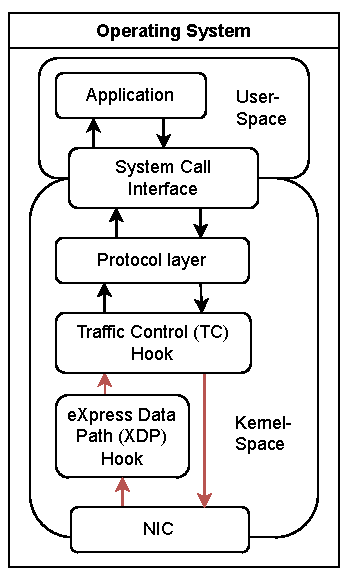
\includegraphics[width=0.3\textwidth]{figures/02_background/hook-point-locations.drawio.pdf}
    \caption[Hook points within network stack]{TC and XDP hook points in the Linux kernel.
    The red loop indicates the ``short-cut'' that the fast-relay utilizes.
    }\label{fig:ebpf-hooks}
\end{figure}

% \subsection{Traffic Control Queuing Disciplines} % TODO: needed?
% The Linux Traffic Control Subsystem uses Queuing Disciplines (qdiscs) to define how packets
% are handled. TODO

\subsection{eBPF Verifier}
Since eBPF programs are executed in the kernel, it is quite obvious that extensive
security checks need to be in place to ensure that the kernel does not experience 
problems like infinite loops, accesses to invalid memory locations, or other security 
related issues.
This explains the existence of the so-called ``eBPF verifier'' which inspects 
every eBPF program for its safety by simulating possible program paths, 
looking at the graph representation of the program and more~\parencite{ebpf-verifier}.
This imposes some restrictions on the complexity of the programs that can be 
used within the kernel.
For our early prototype implementation, this does not cause any issues, since we do not need 
to rely on very complex control structures.
However, if one wants to extend the prototype to support a more complicated packet structure
(e.g.~composition of multiple frames per packet), the verifier might become a limiting factor.


\subsection{Important eBPF Concepts}
One of the most important concepts in eBPF, which we use quite extensively, is 
the ``eBPF-map''.
Such a map boils down to a section in memory that is reserved for the eBPF program
and which can be used as a key-value store for arbitrary data.
This part of memory can then also be accessed from userspace and thus provides the main 
way of communication between the eBPF program and our application.


\vspace{0.5cm}
\noindent\begin{minipage}{\textwidth}
    \begin{lstlisting}[style=CStyle,caption={Examplary eBPF map definitions.}, label={lst:ebpf-map}]
        struct {
            __uint(type, BPF_MAP_TYPE_HASH);        // Hash map
            __type(key, struct client_info_key_t);  // Specific client key
            __type(value, uint32_t);                // 32 bit id
            __uint(max_entries, MAX_CLIENTS);       // Maximum number of clients
            __uint(pinning, LIBBPF_PIN_BY_NAME);    // Pin by name to the tc filesystem
        } client_id SEC(".maps");

        struct {
            __uint(type, BPF_MAP_TYPE_RINGBUF);     // Ring buffer
            __uint(max_entries, MAX_PACKET_EVENTS); // Maximum number of packet events
            __uint(pinning, LIBBPF_PIN_BY_NAME);    // Pin by name to the tc filesystem
        } packet_events SEC(".maps");
    \end{lstlisting}
\end{minipage}
\vspace{0.5cm}

When we define an eBPF-map, we can choose between different types and configure
size, key type, value type, and how the map is stored. % TODO: surely there is more one can define
An example of two eBPF-map definitions can be seen in~\autoref{lst:ebpf-map}.
It shows two different types of maps, a hash map, and a ring buffer, that are used in
our fast-relay setup.
Those and other relevant map types are listed in~\autoref{tab:ebpf-map-types}.


\vspace{0.5cm}

\begin{table}[H]
    \centering
    \begin{tabular}{L{7cm}L{7cm}}
        \toprule
            Type & Description \\
        \midrule
            BPF\_MAP\_TYPE\_HASH & A hash map where keys and values can be arbitrarily defined. \\
        \midrule
            BPF\_MAP\_TYPE\_PERCPU\_HASH & A hash map with separate value slots for each CPU, providing improved performance in multi-core environments. \\
        \midrule
            BPF\_MAP\_TYPE\_ARRAY & An array map that allows random access to elements by index. \\
        \midrule
            BPF\_MAP\_TYPE\_PERCPU\_ARRAY & An array map with separate value slots for each CPU, useful for per-CPU data storage. \\
        \midrule
            BPF\_MAP\_TYPE\_RINGBUF & A ring buffer for implementing high-performance data queues. \\
        \bottomrule
    \end{tabular}
    \caption[Subset of eBPF map types]{Some eBPF map types. (defined in /usr/include/linux/bpf.h)}\label{tab:ebpf-map-types}
\end{table}


\section{Media over QUIC (MoQ)}\label{sec:moq_bg}

\iffalse % TODO: remove (only notes)

Notes on: https://www.ietf.org/blog/moq-overview/

Target: live streaming, real-time collaboration, gaming, etc.

Good scaling capabilities cause high latency
Low latency systems have poor scaling capabilities

MoQ aims for low latency and high scalability
Built on top of raw QUIC (or WebTransport)

Maybe add quote from https://datatracker.ietf.org/wg/moq/about/

Publisher / Subscriber model
Support for many formats, rate adaptation, cache friendly mechanisms, etc.
Relays function as caches for lower latency and higher quality

Took approaches from RTP (real-time stuff), HLS/DASH (scaling)

If many downstream requests for same data, relay only needs one copy

Media content can be end-to-end encrypted but relay can still access metadata
like priority field - this is similar to our setup.
% TODO: how can these fields still be accessed? are they just not encrypted?
Priority can be used when caching or when forwarding under congestion.
The MoQ can drop or delay certain media if necessary.

VoD consumption >> live streaming but live makes up most of peak traffic

MoQ will have great influence on real-time collaboration infrastructure like 
Zoom, Teams, etc.~and live streaming platforms like Twitch, YouTube, etc. 

low latency, high fan out, high scalability is pretty much ideal for most apps.

(Also psychological improvement since latency problems tend to be blamed on the 
other party, not the network.) % TODO: prolly no fit in this section?
https://blog.webex.com/hybrid-work/how-latency-harms-collaboration/

\fi

% \subsection{What is Media over QUIC (MoQ)?} % TODO: maybe not needed
On the application layer we will use the Media over QUIC (MoQ) protocol which 
is as of summer 2024 still being in the process of standardization by the IETF\@.
MoQ targets live-streaming and real-time collaboration applications like Zoom,
Microsoft Teams, or Google Meet.
It is built on top of the QUIC protocol with the possibility of using WebTransport
for browser support.
A general publisher/subscriber model is used and the draft tries to combine
performant approaches from protocols like RTP (for real-time features) and HLS/DASH
(for scalability).

\subsection{Solving Scaling versus Latency}
For a long time now there have been two different camps with regards to media-data-
transmission-protocols and -setups.
One is heavily focused on low latency while the other is aiming for high scalability.
Systems of the former kind include real-time collaboration tools like aforementioned
Zoom, Teams, or Meet.
The latter ones are often huge platforms like Twitch, YouTube or Netflix which need to 
reach millions of users at the same time.
The one thing both have in common is that it turns out to be difficult to incorporate both 
low latency and high scalability into the system at the same time.
The MoQ protocol tries to solve this by providing a setup that is both low-latency and
highly scalable.
To achieve this it supports performance enhancing approaches like relay caching or support 
for adaptive rate mechanisms. % TODO: other things that are used to achieve this?

\subsection{Design of a MoQ Relay}
The charter for the IETF working group describes what MoQ, and therefore also a relay 
that wants to meet the MoQ requirements, needs to support.
These requirements for the publication- and distribution-setup mention the support of 
multiple formats, dynamic rate adaption mechanisms (e.g.~used for congestion handling)
as well as cache-friendly mechanisms.

\begin{figure}
    \centering
    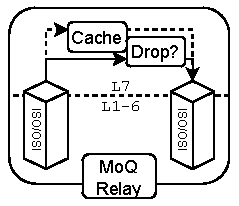
\includegraphics[width=0.3\textwidth]{figures/02_background/moq-relay.drawio.pdf}
    \caption[Rough MoQ relay architecture]{Rough MoQ relay architecture.}\label{fig:moq_relay_architecture}
\end{figure}

Figure~\ref{fig:moq_relay_architecture} gives a visualization of the rough architecture
of a MoQ relay.
It hints at key components like the relay level cache and the congestion handling
mechanism.
What one can also infer is the place of MoQ in the OSI-model namely at the application
layer which itself builds on top of lower level protocols like QUIC, UDP, IP and Ethernet.
In figure~\ref{fig:non_caching_relay_data_request} and figure~\ref{fig:moq_relay_data_request} 
one can see a comparison between the delayed fan-out of the media content caused by the MoQ 
relay and a more traditional setup.
The former is able to reduce the traffic through a network by making multiple transmissions
of the same data between server and relay obsolete.

\begin{figure}[!htb]
    \begin{minipage}{0.45\textwidth}
        \centering
        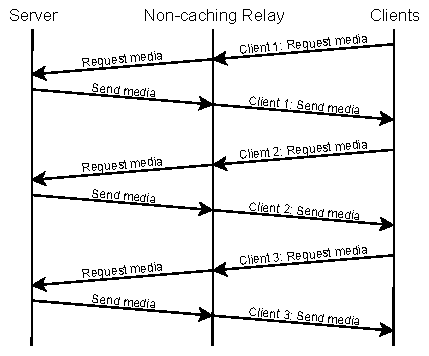
\includegraphics[width=1\linewidth]{figures/02_background/non-caching-relay-data-request.drawio.pdf}
        \caption[Non-caching relay traffic]{Multiple data transmissions for different clients.}\label{fig:non_caching_relay_data_request}
    \end{minipage}\hfill
    \begin{minipage}{0.45\textwidth}
        \centering
        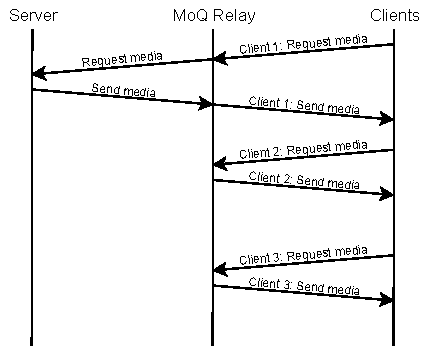
\includegraphics[width=1\linewidth]{figures/02_background/moq-relay-data-request.drawio.pdf}
        \caption[MoQ relay traffic]{Only single data transmission towards the relay.}\label{fig:moq_relay_data_request}
    \end{minipage}
\end{figure}

This caching mechanism fits quite naturally into our proposed eBPF setup since we will need to 
communicate packet data between kernel- and user-space anyway to keep the QUIC library in a 
consistent state.
In addition to that the congestion handling functionality of the MoQ relay can also
be integrated fairly easy within eBPF\@.
This is because packet dropping is ultimately one of the main use cases of plain eBPF 
programs and as such easy to implement.
In a later section will go into detail on how the eBPF setup actually uses mechanisms like 
priority fields for this and how those meet the standard specifications.

\subsection{moqtransport}
In order to use the MoQ protocol in our setup we will make use of a library that implements 
the MoQ transport protocol (moqtransport or MoQT) in Go~\parencite{priority-moqtransport-repo}
The goal of MoQT is to define a media transport protocol that is operating on top
of QUIC and WebTransport which is providing the concrete designs that the charter of 
the MoQ working group is aiming for.
This includes, for example, actual structure of the different message types or error handling in case 
of a wrong state.
As of writing this thesis the MoQT draft is in its fifth version~\parencite{draft-moqtransport}.

% Besides that the fast-relay implementation will also make use of the moqtransport library.
% This library brings the `Media over QUIC' (MoQ) protocol to Go and will be used as a media transport protocol 
% when looking at the impact of fast-relays on adaptive real-time video streaming.
% The MoQ protocol is being standardized by the IETF since July 2023 and has yet to be finalized. 
\section{Real Time Communication and Adaptive Bitrate Streaming}\label{sec:rt_and_adaptive_bitrate_streaming}

Whenever we look at different types of streaming it is important to consider the 
different requirements that come with them.
We differentiate between a one sided communication, where an increase in delay 
in order to gain a higher quality is acceptable, and a two sided communication, 
where a low delay is crucial for satisfactory user experience.
The former allows for more complex setups like the one considered in subsection
\nobreakspace\ref{subsec:adaptive_bitrate_streaming} while the latter requires
a more direct approach which will be discussed in the following subsection.

\subsection{Real Time Communication}
When looking at streaming setups that consider real-time constraints, such as conferencing 
where interhuman communication is involved, the objectives of the connection tend towards
low latency.
In order to provide natural feeling human communication, the delay between the sender 
and the receiver has to be minimal.
This type of communication between devices is often referred to as ``Real-Time Communication'' 
(RTC) and used in many applications, such as Zoom, Skype, or Discord.

\subsubsection{Mechanisms and Ideas}
The main goal of such systems is to minimize the delay between the sender and the receiver
while additionally allowing all parties to communicate with each other.
A lot of design decisions are made with this in mind.
One design decision for a large conferencing system like Zoom
might consider the usage of peer-to-peer (P2P) connections versus a server-based
approach.
While P2P might allow for lower latencies in case of a small number of participants,
a server-based approach scales a lot better and can therefore provide a better
ressource utilization.

\subsubsection{Implications on Streaming Setup}
The need for low latency also has implications of the specific setup at hand.
An example of such an implication is the design of the connection between the 
real-time connection network (RTCN) and a client.
Since retransmissions are expensive in terms of latency, a setup should strive to minimize 
the distance a packet has to travel through an unreliable network.
This could be achived by having multiple, strategically placed, eddge-servers, which internally use 
a, compared to the internet, more reliable connection, for longer (e.g.~intercontinental) connections.
This way packet loss occuring during the client-to-edge-server connection would not have a big 
impact on the overall latency of the connection.
A visualization of such an appraoch can be seen in~\autoref{fig:real-time-streaming-connections}.

\vspace{0.5cm}
\begin{figure}[H]
    \centering
    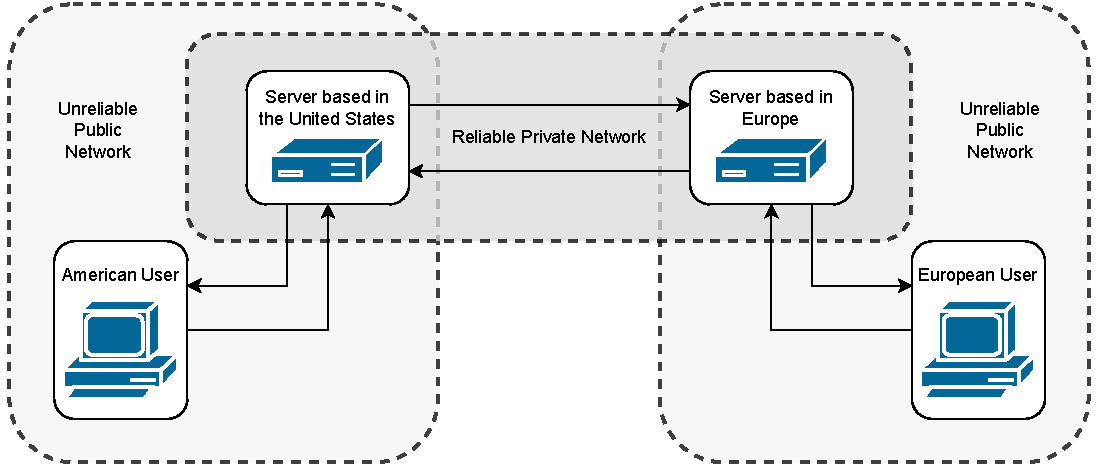
\includegraphics[width=0.8\textwidth]{figures/02_background/real-time-streaming-connections.drawio.pdf}
    \caption[Real-time streaming connections]{A setup with multiple edge-servers around the world
    can help to minimize the latency of a connection.}\label{fig:real-time-streaming-connections}
\end{figure}

\subsection{Adaptive Bitrate Streaming}\label{subsec:adaptive_bitrate_streaming}
Multimedia streaming is a big part of the internet and many optimizations have
been developed to improve the quality of service for the end-users.
This includes considering (in real-time) parts of the clients' connection state, 
such as available bandwidth, and adapting the rate at which a server sends data.
Such a process is called ``Adaptive Bitrate Streaming'' (ABS) and is employed in many 
of today's streaming setups.

% TODO: cite    https://netflixtechblog.com/optimizing-the-netflix-streaming-experience-with-data-science-725f04c3e834
% TODO:         https://www.cloudflare.com/de-de/learning/video/what-is-adaptive-bitrate-streaming/
% TODO:         https://docs.imagekit.io/features/video-transformation/adaptive-bitrate-streaming
\vspace{0.5cm}
\begin{figure}[H]
    \centering
    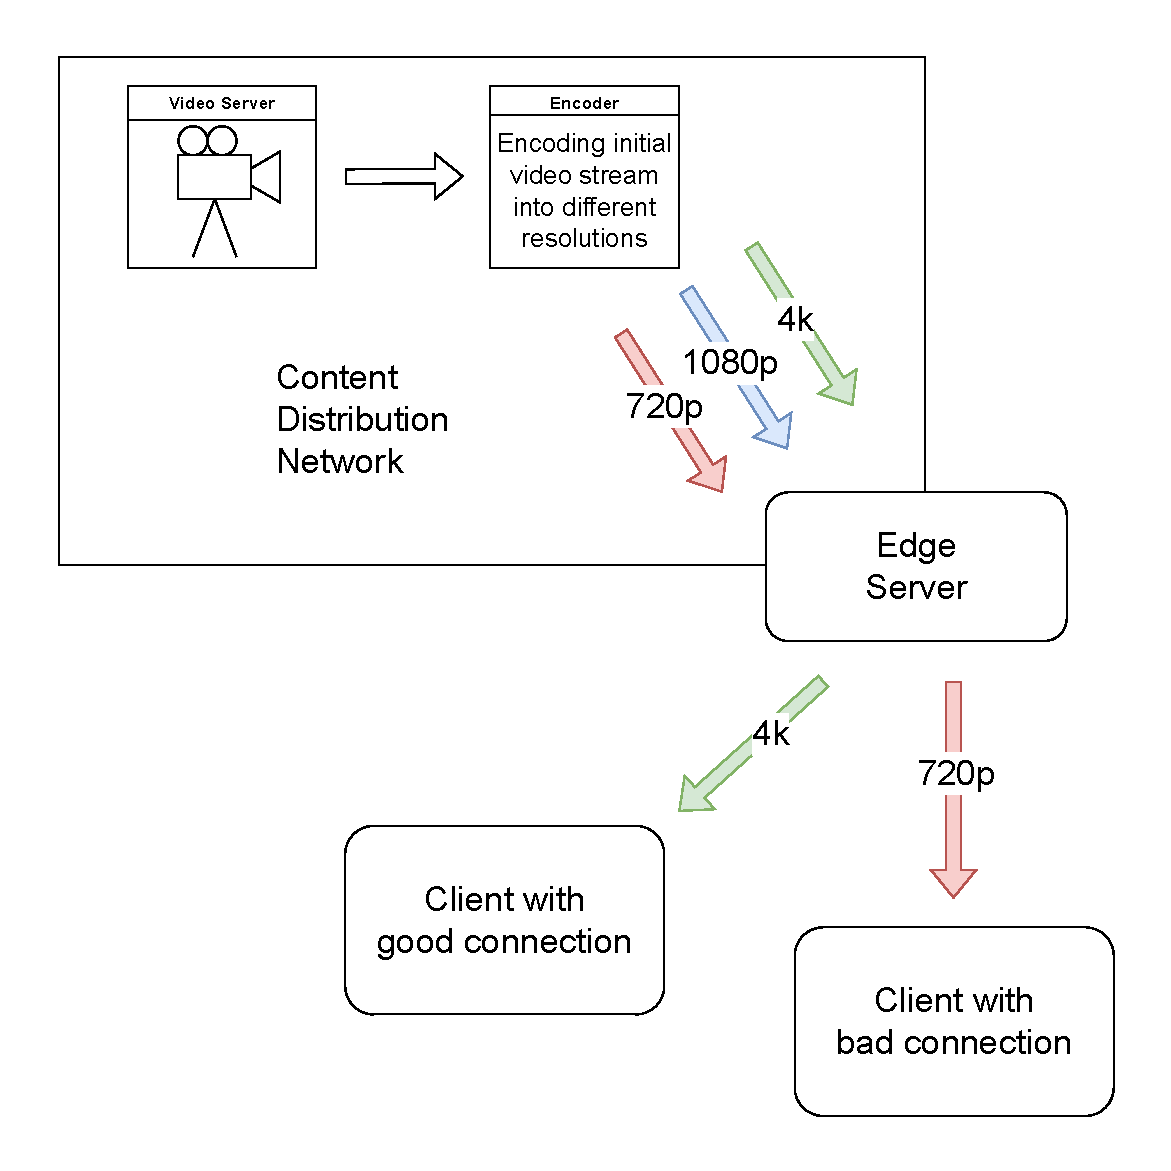
\includegraphics[width=\textwidth]{figures/02_background/adaptive-bitrate-streaming.drawio.pdf}
    \caption[Adaptive streaming schematic]{Behind the scenes multiple streams with different
    resolutions exist to allow adapting to a user's bitrate.}\label{fig:adaptive-bitrate-streaming}
\end{figure}
% The way the example implementation of fast-realys in this thesis is set up,
% is that the video server will encode into each packet its priority.
% For example I-frames have a high priority while P-frames have a lower
% priority.
% The relay then can decide not to forward certain packets to a client if
% the client is experiencing congestion.
\vspace{1cm}

\subsubsection{Mechanisms and Ideas}
ABS implements the simple idea of changing the amount of data sent to a client 
based on the clients' connection quality.
This means a client with a good connection gets a higher-quality stream than 
one with a bad connection.
For this, the internal setup needs to be able to provide multiple streams with
different resolutions and bitrates.
An example setup can be seen in~\autoref{fig:adaptive-bitrate-streaming} where
an encoder creates streams with different resolutions and an edge server, that 
manages the connections to the clients, can switch between those streams based on
the connection state of a specific client.
Twitch and YouTube-Live are examples where, although more complex, similar setups
are used to provide a better user experience.
The premise of such a setup is that in case of a bad connection, it is still 
preferable to be able to watch a stream continuously, even if that means
cutting down on quality.
When looking at such real world examples, however, it is important that one keeps 
the differences between Video-on-Demand (VoD) and live-streaming in mind.
The latter might require more computation before a video is sent since the media 
has to be processed on the fly since it is created in real-time.
For VoD on the other hand the media already exists in its final form. 

\subsubsection{Implications on Streaming Setup}
ABS forces a few changes to the way servers and relays are set up.
First, as figure~\autoref{fig:adaptive-bitrate-streaming} shows, there needs to 
be an ``encoding'' component that turns the single, high-quality stream that is 
received from the streaming source into multiple streams with different resolutions.
Besides that, the relay needs to keep track of the clients' connection quality, e.g.~using 
measurements like RTT, packet loss, etc., and decide which stream to forward to the client.
Since the connection quality can change dynamically the relay also needs to continuously
monitor each connection and potentially change the used stream.
Besides encoding and monitoring aspects the system also has increased storage requirements
since stream data will essentially be duplicated.

\section{Related Work}\label{sec:related_work}

Our approach combines ideas from multiple different 
related publications.
This section will give a brief overview of some related work 
that uses similar concepts such as packet handling using a BPF 
program or bypassing the Linux network stack to improve performance.

\subsection{eQUIC Gateway}
There have been previous publications on making QUIC more efficient by using BPF programs
such as~\parencite{equic-gateway}, where a BPF program is used together with the Linux
eXpress Data Path (XDP) to filter packets based on information provided by the userspace.
This approach provided significant performance improvements with an increase of throughput
by almost a third and a reduction of CPU time consumption caused by filtering packets by
more than 25\%.
This shows that a setup leveraging Linux kernel features such as BPF has a lot of potential
to improve the current infrastructure.
% TODO: more specific info on how this paper's setup looks like / differs from ours?
% TODO: mention that XDP is not feasible for our setup because it has no egress hook?

\subsection{Kernel Bypass}
Another interesting approach that follows a similar idea of speeding up packet processing
by avoiding the Linux network stack is~\parencite{kernel-bypass-msc-thesis}.
The difference in this work is that DPDK is used to bypass the network stack to 
then process packets in userspace instead of directly using eBPF programs for processing,
as we do.
This, for example, offers more flexibility as the userspace program is not as limited (e.g.\ 
by the eBPF verifier) as the eBPF program but might also lead to slightly more system calls,
especially in the setup of a system, when user- and kernel-space need to communicate, thus 
increasing latency.
% TODO: clear enough / everything covered and correct?

\subsection{Priority drop}
The idea of dropping packets based on their priority to adapt a connection
in a congestion event has also been around for a while.
This is explored further in~\parencite{media-streaming-prio-drop}.
There the authors discuss a more tailorable congestion handling 
compared to video quality discretization as well as an improvement 
to, potentially randomized, frame dropping.
This thesis, similar to~\parencite{media-streaming-prio-drop}, will not focus
on how the priority for a specific packet is determined but rather on how
packets are handled in general.
For this, it is assumed that a higher-level protocol has correctly determined 
the packet priorities and can handle the drop of packets with lower priority
in case of limited bandwidth.
% TODO: explain more on different ways of encoding priorities e.g. I- and 
% TODO: P-frames in video streaming?
\section{Summary}\label{sec:summary_ch2}

In this chapter we have introduced some prerequisites for the 
upcoming one.
We have looked at the QUIC transport protocol and the MoQ protocol, which is 
based on top of QUIC\@.
We have also mentioned eBPF and presented two different concepts in the 
realm of streaming, namely ABS and RTC\@.
In the next chapter, we will combine these concepts to create a 
relay design that is capable of traffic forwarding.
We will do so by first mentioning necessary changes to the library 
implementing the QUIC standard, then we will explain our proposed eBPF setup 
and finally, we will go into detail on special considerations like 
userspace synchronization or congestion related topics.
\newpage
% !TeX root = ../main.tex
% Add the above to each chapter to make compiling the PDF easier in some editors.

\chapter{Fast-Relays}\label{chap:fast_relays}

In this chapter, we will dive into the specifics of our proposed fast-relay setup.
We will cover necessary library adaptations as well as setup specifics like eBPF programs 
and userspace synchronization.
Figure~\ref{fig:route-layering} shows a high-level overview of a basic 
server-relay-client setup with its respective networking layers.
A conventional setup would have the packet travel into userspace at the relay, 
while our setup aims to reduce the critical path, as indicated by the red arrows.

\vspace{0.5cm}
\begin{figure}[htbp] % TODO: where to put this?
    \centering
    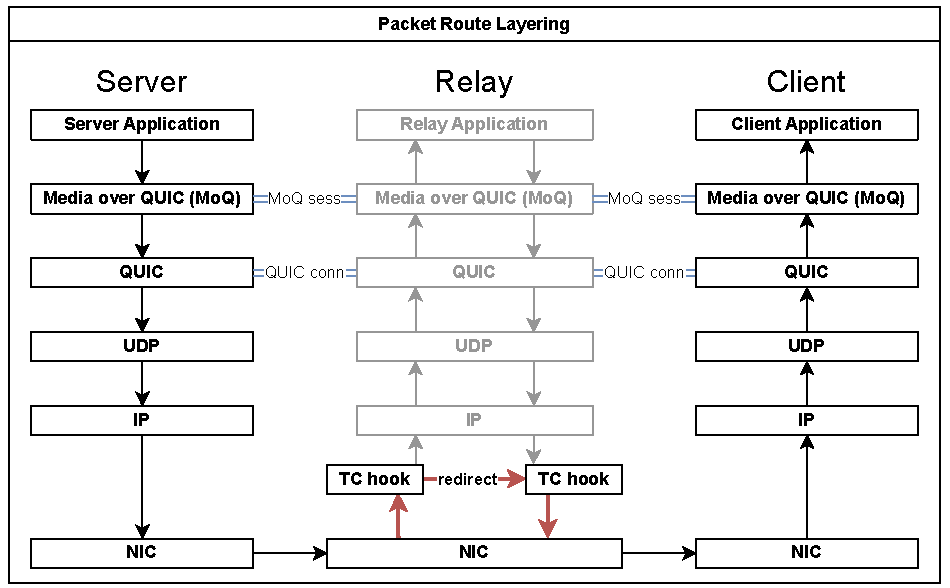
\includegraphics[width=0.7\textwidth]{figures/03_fast_relays/route-layering.drawio.pdf}
    \caption[Packet path schematic regarding network stack]{Conventional networking layers a packet passes.
    The red loop indicates again the ``short-cut'' that is utilized by the fast-relay 
    (eBPF packet-forwarding {-} no need to go up to userspace).}\label{fig:route-layering}
\end{figure}

\section{QUIC Adaptions}\label{sec:quic_adaptions}
As was already mentioned in the previous chapter, our setup requires some adaptations
to the quic-go library.
One initial change necessary was to turn off packet en- and decryption, 
that is happening within quic-go.
Given that we operate on the QUIC-header data within the eBPF program, we need access 
to fields that are encrypted using QUIC header-protection.
For obvious reasons sending unencrypted packets is not something that would be wanted in 
a production environment, but for our exemplary setup, it is unproblematic. 
An alternative would be to ``push down'' en- and decryption onto a smartNIC using a 
hardware offload, but at the time of writing, there was no such offload available for QUIC\@. 
Given that such a hardware offload is added in the future, the en- and decryption can be
turned on again, which makes this change more of a temporary solution to show the feasibility
of our approach.

\subsection{Function-Pointer Style Additions}
Another type of change that we needed to introduce into the quic-go library is caused by 
connection state management.
We essentially added support for communication with the eBPF program by using an 
approach similar to C-style function pointers.

On multiple locations, we added conditional function calls like the one depicted in 
\autoref{changes:function-pointer}.
The function that is called here will be defined by the developer of the relay and 
therefore allow for customizability without the need for changing the library itself.

\vspace{0.5cm}
\noindent\begin{minipage}{\textwidth}
\begin{lstlisting}[style=GoStyle, label=changes:function-pointer, caption=An example of a function-pointer addition to the quic-go library.]
    /* Function pointer call within actual quic-go code */
    if packet_setting.ConnectionUpdateBPFHandler != nil /* && potentially other conditions */ {
	    packet_setting.ConnectionUpdateBPFHandler(connId.Bytes(), uint8(connId.Len()), p.connection)
	}
\end{lstlisting}
\end{minipage}

\vspace{0.5cm}
\noindent\begin{minipage}{\textwidth}
\begin{lstlisting}[style=GoStyle, label=changes:signature-function-pointer, caption=Only the signature will be defined within the library itself.]
    /* Function pointer signature definition within additional config file */
	ConnectionUpdateBPFHandler      func(id []byte, l uint8, conn QuicConnection) = nil
\end{lstlisting}
\end{minipage}

The definition of the function that the developer of the relay wishes to be executed at specifically
defined points will be defined locally in the relay code and provided to the configuration of the quic-go library.
An example of how this could look like is shown in \autoref{changes:definition-function-pointer}.

\vspace{0.5cm}
\noindent\begin{minipage}{\textwidth}
\begin{lstlisting}[style=GoStyle, label=changes:definition-function-pointer, caption=An example of how the addition looks on the relay side.]
    /* Definition of the function within the local relay code */
    func localUpdateConnectionId(id []byte, l uint8, conn packet_setting.QuicConnection) {
        /* handle the connection update by interacting with the eBPF program */
    }   

    /* Providing the function to the quic-go library */
    func main() {
        /* ... */
        packet_setting.ConnectionUpdateBPFHandler = localUpdateConnectionId
        /* ... */
    }
\end{lstlisting}
\end{minipage}

The need for these additions arises since the eBPF program works with its own copy of the current state of a connection.
This, for example, includes the connection-id that will be used when changing the packet header before sending it out.
Since a connection-id can change, i.e.~be updated or retired, during the lifetime of a connection, we need a way to inform 
the eBPF program to no longer use outdated state-information.
These function-pointer style additions provide a minimal way of adding such functionality without limiting flexibility 
or adding too much application-specific code to the library itself, as would be the case if the library would access 
the eBPF-Maps directly.

% TODO: mention changes which are not function-pointer style
\subsection{Direct Changes to the Library}

\iffalse
% open stream with priority (+ datagram)

% turn off crypto (reaction to CRYPTO_TURNED_OFF flag)

% connection-id retirement specific stuff (switch to priority id)

% fixed sizes for fields e.g. conn id, stream-id, etc.(just for ease of development)

% e.g. only single stream frame inside packet (for ease of development) since general approach too complex for verifier?

% retransmission functions that open new stream with correct id

% registerBPFPacket function for connection

% prio enum. (prolly could be also given by relay dev) % TODO: not interessting enough i'd say
\fi

Besides the simple function-pointer style additions, we also had to make some direct changes to the library.
These include simplifications of the packet structure to make the implementation of a prototype easier 
but also changes that are necessary for the whole approach to work.
The necessary state changes mainly required internal state adjustments that would not be possible from outside 
the library because of missing access/visibility.
The optional turn-off for the packet en- and decryption based on the value of the \verb|CRYPTO_TURNED_OFF| flag
also required some direct changes to the library, but these will not be mentioned further since they are temporary
and not a focus of this chapter.

\subsubsection*{Simplifications of Packet Structure}
We added some changes to the quic-go library to make a prototype implementation easier.
The first one is that we fixed the sizes of some variable length fields like the connection-id or the stream-id.
This was mainly to avoid the need to figure out the correct sizes within the eBPF program as this would have 
resulted in approaches that would have to be very carefully turned into eBPF-compatible code due to verifier
restrictions.
Besides fixing the length of some fields, we also limit the number of frames per packet to one.
Normally a QUIC packet can contain multiple frames, especially stream-frames, but this would have required 
a packet traversal within the eBPF program that, again, would have been harder to implement considering all
verification constrictions.
Besides this additional complexity, for our usecase the ``singe-stream-frame-per-packet'' approach is not changing
a lot since the payload of one media packet will be split into multiple packets due to its size.
This means a single stream frame is likely already using up a whole packet, and multiple frames per packet would 
not be happening.

\subsubsection*{Stream Priorities}
Our approach relies on the fact that every packet has a priority value assigned to it.
In our case this priority value is stored within the connection-id.
Based on this, the first change, which is not only for simplification of our prototype implementation but is actually needed for 
our approach to work, is the addition of opening a stream with a specific priority.
Our assumptions define that the server is the one marking the packets with the correct priority, which in 
our case is realized by sending them over a specific stream.
Every stream is bound to a specific priority value, and our code changes will make sure that the connection-id
that is used for any packet sent on this stream will contain the correct priority value.
Figure~\ref{fig:priority-stream} visualizes the setup as well as our rudimentary approach of saving the 
priority value as the first byte of the connection-id.

\vspace{0.5cm}
\begin{figure}[H]
    \centering
    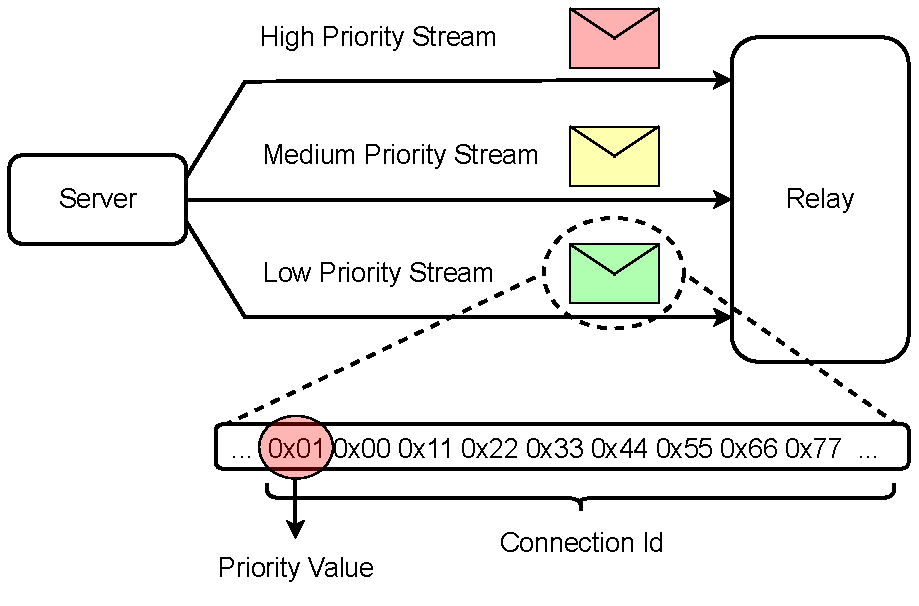
\includegraphics[width=0.7\textwidth]{figures/03_fast_relays/priority-streams.drawio.pdf}
    \caption[Streams with specific priorities]{The server opens streams with specific priorities, 
    which are then used to send packets with the corresponding priority.}\label{fig:priority-stream}
\end{figure}

This approach of having the priority value saved within the connection-id caused the need for another 
change in the library.
Due to the periodic change/retirement of connection-ids, we need to make sure that at any point in time, there 
exists one connection-id for each priority within the connection.
Otherwise, we might be unable to mark a packet with the correct priority.
This led us to introduce some additional logic to the code that is executing the retirement of connection-ids.
There, we will make sure that before a connection-id is retired, either one with the same priority value
already exists or is created.
This solves the problem of not being able to mark a packet with the correct priority.

\subsubsection*{Retransmission}
Another direct change that is needed is that of a specific \verb|OnLost| function for packets that 
have been forwarded by the eBPF program.
Since the relay state is not necessarily aligned with the server state, and the relay does not know
about the stream a packet was sent on, it is not possible to reuse the plain \verb|OnLost| function
of the quic-go library.
This is because the plain \verb|OnLost| function would lookup the stream corresponding to the provided stream-id and 
retransmit the packet on there, but the stream for the given id might not exist within the relay stream-pool.
Instead, our new function needs to look up the stream-id of the lost packet and open a new stream with
the same stream-id, ensuring that the client correctly receives the retransmission.
Besides the stream-id, the created stream-object should also have the same remaining stream-state
as the original stream (e.g.~offset-information).  
When a retransmission happens, the relay also needs to tell the underlying eBPF program that a packet is part of a 
retransmission and that, even if a stream was actually created by the relay, the egress program should treat it like 
it was created by the server.
That last part is necessary for the stream-id translation part of the egress program, which is explained further
in section\nobreakspace\ref{sec:client-egress}, to work correctly.
This functionality of informing the eBPF program about the retransmission, however, is again realized by a 
function-pointer style addition and thus designed by the relay developer.

\subsubsection*{Visible Endpoint for Packet Registration}
The last direct change that we added was the introduction of an additional function \verb|RegisterBPFPacket| 
on a quic-go connection object that allows the relay to register a packet.
Since the packet registration requires access to internal state of the connection, this also needed to be 
done as an actual change to the library.
Now the relay can just read the necessary information of a packet that needs to be registered
from the eBPF-maps and then pass it on to this function which will handle the registration.
This also provides a good separation between the Go code that handles eBPF communication and the actual
QUIC connection handling.
\section{eBPF Setup}\label{sec:ebpf_setup}
\subsection{Different eBPF Programs}
\begin{figure}[htbp]
    \centering
    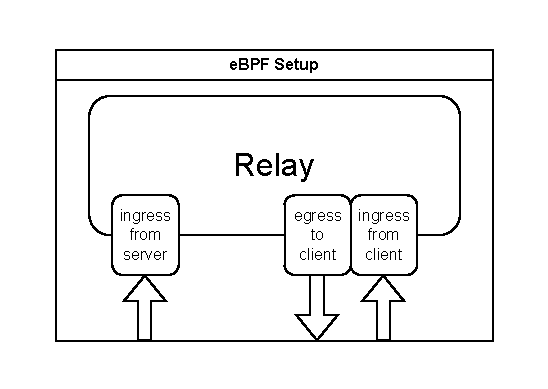
\includegraphics[width=0.3\textwidth]{figures/03_fast_relays/ebpf-setup.drawio.pdf}
    \caption[Types of eBPF programs at relay]{The relay has to be equipped with three BPF programs.}\label{fig:ebpf-programs}
\end{figure}

In order to allow the relay to forward packets independently of the userspace, we
need to equip the relay with three BPF programs as seen in figure.
Those three programs are 
\begin{itemize}
    \item a program that handles incoming traffic \textbf{from} the clients (client ingress),
    \item a program that handles outgoing traffic \textbf{to} the clients (client egress) and
    \item a program that handles incoming traffic \textbf{from} the video server (server ingress).
\end{itemize}
Their responsibilities then are
\begin{itemize}
    \item handling the initial registration of new clients and storing their information such as
    MAC addresses in a BPF map,
    \item intercepting the packets from the video server, duplicating and redirecting them to 
    the egress program (as well as sending one unaltered packet to userspace for state
    management purposes),
    \item receiving the redirected packets at egress, altering them using the client specific
    data, deciding (based on packet priority and client congestion) if a packets should be dropped 
    or sent, storing info on sent out packets for future congestion control purposes and finally sending 
    them out to the clients.
\end{itemize}
This setup allows us to separate any state management and congestion control from the actual
packet forwarding and thus makes leaving out any immediate userspace processing possible.

Following is a more detailed description of the responsibilities of each of the three programs.
\subsubsection{Client Ingress} 
The ingress eBPF program initially does some simple packet inspection on every incoming packet 
looking if the packet uses the correct protocols and addresses the right application layer.
This is done by initially parsing the Ethernet, IP and UDP headers, if present, and checking if 
the port matches the listening port the relay application is listening on.
This means the correct port is to be defined prior such that the eBPF program can associate 
a single or (multiple) relay instance(s) with the correct port.
In our case then, since we use QUIC, the program will check for QUIC long header packets that 
setup an initial connection and saves the transmitted state information such as connection id, 
stream related states, etc.~in an eBPF map together with information that is not directly known
by the userspace such as the MAC address of the client.
Saving data like the MAC address directly once the connection is set up allows to omit any further 
Address Resolution Protocol (ARP) steps later on. 
\subsubsection{Server Ingress}
Another ingress related program, this time for packets coming from the video server, is needed
to handle packet duplication and forwarding.
This program will receive the actual video packets from the server and then, based on an internal 
counter of how many clients actually want to receive the video, duplicate the packet accordingly.
The counter of clients will be updated by the userspace once a new connection is fully established
and the client is ready to receive the actual video data.
This might potentially cause some miniscule delay when updating the counter but sending cached 
video data to the client for a brief moment when updating the counter could be a solution for that. % TODO: needed?
Figure~\ref{fig:packet-forwarding-duplication} shows the packet duplication and forwarding process 
high level for an example setting with three clients that want to receive the video data.
In the ingress program from the server we need to consider a few things to ensure the correctness
of our approach.
These are:
\begin{enumerate}
    \item   The program can \textbf{only} forward packets that containing video data and must not 
            forward any other packets that contain e.g.~control data.
    \begin{enumerate}
        \item   This is fairly easy to achieve by doing some header inspection of the QUIC header
                which contains the packet type. Also since payload is generally sent using 
                0-RTT- (i.e.~short-) headers there is no need to consider long-header packets.
    \end{enumerate}

    \item   The program should pass an unaltered copy up to userspace to allow the QUIC library to
            gain knowledge of the packet and handle any state changes accordingly.
    \begin{enumerate}
        \item   Generally speaking this is not strictly necessary as one could just have a separate 
                setup of registering packets that came from the server but as this is not needed
                it is considerably easier to just pass the packet up to userspace and let the 
                library handle it normally. This does not impose any additional overhead as the
                forwarding of any duplicate packets happens independently of course.
        \item   Any packet that has been identified as not part of our dataflow should of course 
                be passed up to userspace without being forwarded to egress.
    \end{enumerate}
\end{enumerate}

\begin{figure}[htbp]
    \centering
    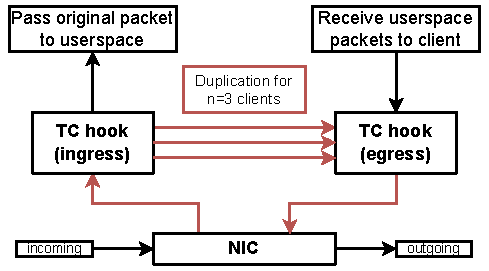
\includegraphics[width=0.5\textwidth]{figures/03_fast_relays/packet-forwarding.drawio.pdf}
    \caption[Video packet duplication]{Duplication and forwarding of video packets to egress directly 
    from ingress.}\label{fig:packet-forwarding-duplication}
\end{figure}

Duplicating and forwarding incoming packets happens using that were identified as payload 
can be done using \verb|bpf_clone_redirect(skb, egress_ifindex, 0)| which is a helper function
that allows one to clone the packet buffer provided as the first argument and add it to the 
queue of the interface that is provided as the second argument.
The last argument allows to specify additional flags.
Aside from \verb|bpf_clone_redirect| there are also other helper functions regarding packet
redirection with slightly different behavior so it is crucial to choose the appropriate one
to get the desired outcome.
Table~\ref{tab:skb-redirection} shows them together with a brief description of their behavior:

\begin{table}[htbp]
    \centering
    \begin{tabular}{L{7cm}L{7cm}}
        \toprule
            Helper & Description \\
        \midrule
            \verb|bpf_clone_redirect| & Clones and redirects a packet to the interface associated with the provided index.\\
        \midrule
            \verb|bpf_redirect| & Redirects a packet to the interface associated with the provided index. The packet is not cloned 
                                    (no underlying call of \verb|skb_clone()|) so it is slightly more efficient (25\% pps increase according 
                                    to commit message). The packet is also not redirected immediately but after the function finishes.\\ % TODO: find commit message
        \midrule
            \verb|bpf_redirect_peer| & Similar to \verb|bpf_redirect| but instead of redirecting the packet to the interface provided 
                                        as a parameter it is redirected to its peer device. This works only between different netns to 
                                        allow for an efficient ``ingress to ingress netns switch''. The switch is more performant since 
                                        the packet does not need to go through the CPU backlog queue.\\ % TODO: what does the CPU backlog queue do?
        \midrule
            \verb|bpf_redirect_neigh| & Again similar to \verb|bpf_redirect| but allows to redirect a packet to another net device. 
                                        This helper does also fill in all the correct L2 addresses of the neighboring subsystem. 
                                        Internally this executes a neighbor lookup to find the needed L2 information. \\
        \bottomrule
    \end{tabular}
    \caption[Redirection helpers for packet buffer]{Helper functions for packet redirection.}\label{tab:skb-redirection}
\end{table}
% TODO: ^^^^^^^^^^^^^^^^^^^^^^^^^^^^^^^^^^^^^^^^^^^^^^^^^^^^^^^^^^^^^^^^^^^
% TODO: cite this: https://man7.org/linux/man-pages/man7/bpf-helpers.7.html
% TODO: cite this: http://arthurchiao.art/blog/differentiate-bpf-redirects/ ???
Based on the descriptions of the redirection helper functions mentioned in table~\ref{tab:skb-redirection}
it becomes clear that \verb|bpf_clone_redirect| is the only suitable for our use case. 
This is becaus we need the cloning aspect since we essentially want to duplicate the incoming packets multiple times.
Also the redirection to another namespace or another net device as provided by \verb|bpf_redirect_peer| and
\verb|bpf_redirect_neigh| respectively is not needed in our case since we operate in the same relay-namespace
throughout the whole process.

\subsubsection{Client Egress}
The central part of the eBPF setup where all the state-management and forwarding of the other 
eBPF programs comes together is the program that handles the outgoing traffic towards the clients.
The client egress program sees every packet that leaves the relay, which includes packets that have 
been redirected by the ingress program as well as packets that have been generated by the relay itself
(i.e.~come from the relay userspace).
This means that the program essentially merges two streams of packets into one stream that needs to 
be in a consistent state.
This interleaving of packets grows the requirements of the program to the following list.
Bold numbers indicate that a requirement is caused by the interleaving of packets.
\begin{enumerate}
    \item[1.]   Obviously, similar to the other eBPF programs any packet that is not part of our traffic 
            should be passed on normally without any further processing.
    \item[\textbf{2.}] In case the packet is QUIC (for the correct client connection) the packet number 
            needs to be changed to a program internal counter to avoid issues of reusing packet numbers. 
            This is the only place where we can guarantee sequential packet numbers since neither 
            userspace nor the server know what the highest packet number sent at any moment in time is. 
            As there is no way of synchronizing lookups (e.g.~using eBPF maps) of information between userspace 
            and eBPF program changing it right before sending it out is the most efficient way. 
    \item[\textbf{3.}] In case the packet (additionally to being QUIC for a client connection) contains 
                        stream frames we need to do a similar translation of the stream id.
                        Reasons and methods for this are the same as for the packet number translation.
                        Figure~\ref{fig:stream-id-translation} shows a flow diagram of the stream id translation
                        process.
                        Important steps include checking if the stream id translation is already existing as well
                        as checking if the packet is a retransmission.
                        The former is necessary in case a payload is split into multiple packets and the latter is 
                        necessary since the retransmission physically come from the relay but should be treated as 
                        if they came from the server.
    \item[4.] Again in case the packet is QUIC and for the right connection the program needs 
                        to read the priority of the packet and decide via map-lookup if the connection 
                        allows for sending packets with the given priority.
    \item[5.] In case the packet is a redirected media stream data packet the program needs to find out 
            which client is the receiver. 
            This is done by saving the client id in some part of the packet that will be overwritten 
            at egress (namely the connection id) before redirecting the packet.
            The egress program, knowing where the id is saved in case of a redirected packet, can then
            lookup the correct address data of the client (i.e.~MAC address, IP address, etc.) and
            overwrite the respective fields in the buffer before sending it out.
\end{enumerate}
\vspace{0.5cm}
\begin{figure}[H]
    \centering
    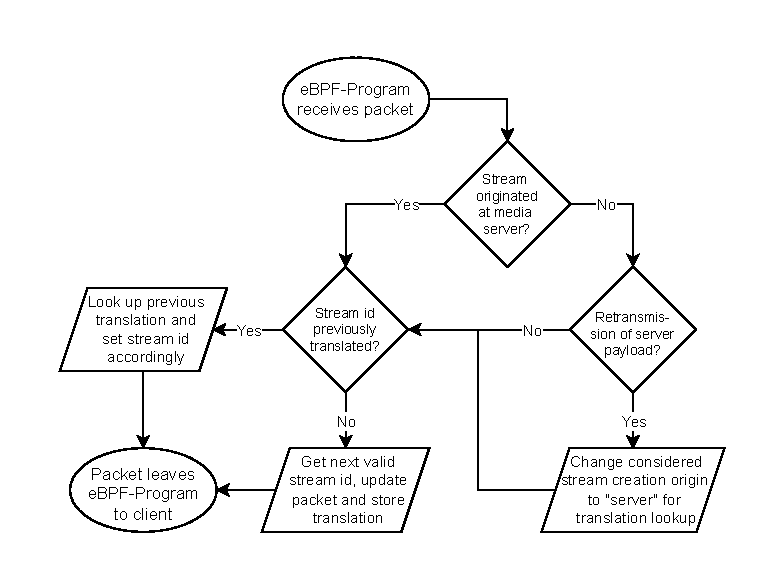
\includegraphics[width=0.7\textwidth]{figures/03_fast_relays/stream-id-translation.drawio.pdf}
    \caption[Stream id translation schematic]{Flow diagram of stream id translation process.}\label{fig:stream-id-translation}
\end{figure}
% Since the QUIC protocol works with packet numbers for a given connection it is necessary for 
% the egress program to make sure the forwarded packets together with the userspace packets
% provide a consistent state. 
% For this the egress program maintains its own packet number counter for each connection.
% That way only one counter has to be maintained and race conditions can be avoided.
The aforementioned packet number translation means that the packets sent by the userspace are 
likely to have a different packet number than the one chosen by the QUIC library.
This might lead to inconsistencies again when receiving acknowledgements but can be avoided by 
remembering the translation in a map as well as storing only packet-objects in the 
Go library that have the correct state.
This technique of ``storing'' a packet that the userspace either has sent itself or does not know
about since it comes from the media server will be referred to as ``packet registration''.
This initially gives a brief window where a packet was sent out but is not saved in the history
of the QUIC library but once the packet is then processed by the userspace routine handling the 
registration, any incoming ACKs for this packet can be processed correctly.
The next section will go more into detail on how the packet registration works.
Later we will also look at the implications of sending a packet the library does not know on 
retransmissions.
Even though the stream id translation works very similar to the packet number translation it 
does not have the need for any additional work after the packet has been sent out since our 
approach uses unidirectional streams only and thus the relay does not care about changes in 
the used stream id. % TODO: maybe reorder the sentences a little bit

\subsection{Packet Registration}
In order to make the congestion control algorithm that is running in userspace
usable we need to inform the QUIC library about the forwarded packets.
This again happens via BPF maps and a separate go routine that continuously
polls new entries in the map and processes them.
Entries are then added to the packet history to allow the receipt of ACKs.
Besides that, the congestion control algorithm will be informed about the
forwarded packet in order to be able to react to potential congestion events.
Figure~\ref{fig:forward-registration} visualizes the setup for this process.
\begin{figure}[H]
    \centering
    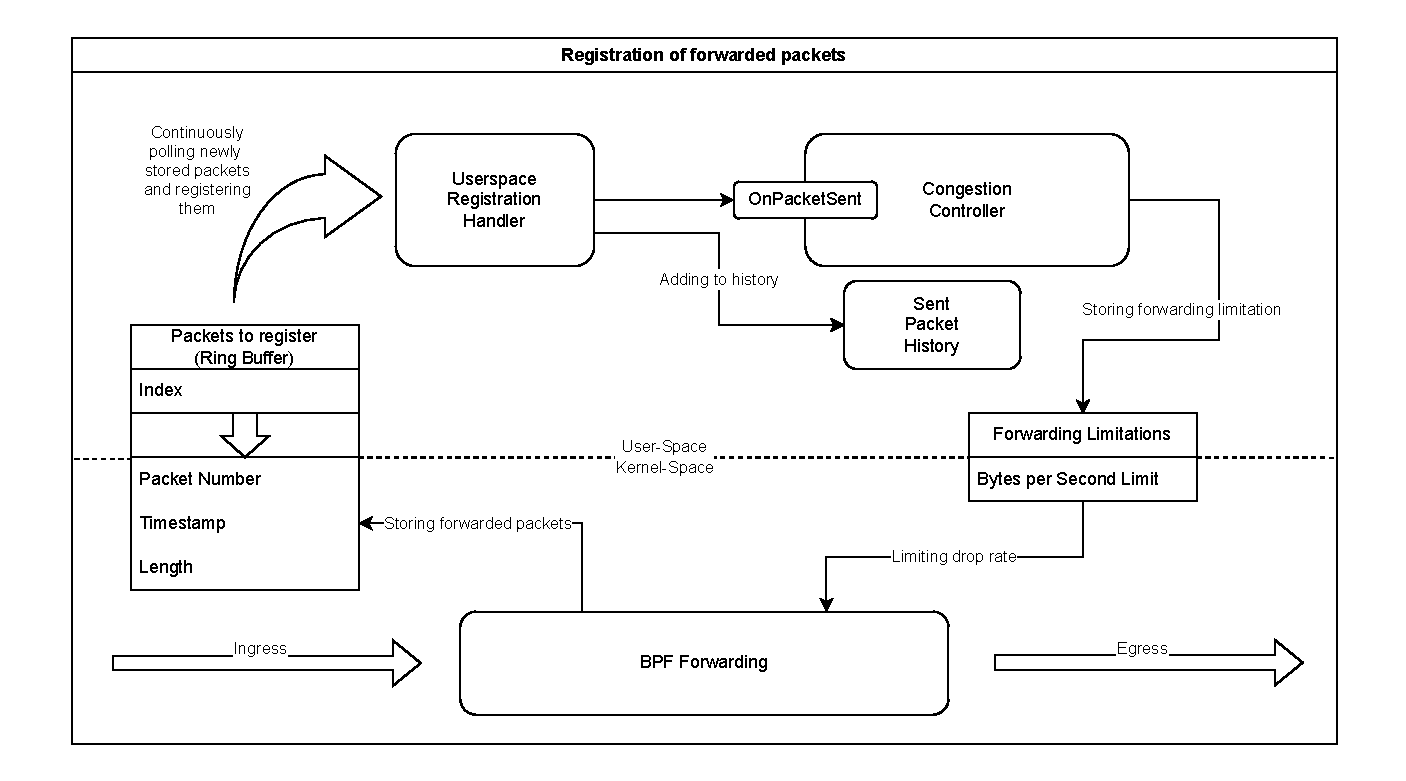
\includegraphics[width=0.7\textwidth]{figures/03_fast_relays/forward-registration.drawio.pdf}
    \caption[Packet registration schematic]{Internal setup for registering forwarded packets as well as incorporating forwarding
    limitations for the BPF program.}\label{fig:forward-registration}
\end{figure}

\subsection{Retransmissions of Forwarded Packets}
TODO

\section{Userspace Synchronization}\label{sec:userspace_synchronization}

Since one of the main ideas we propose is to avoid passing a packet all the way
through the network stack up to userspace at the relay, we create the 
problem that the application itself is not aware of packets that 
are being sent.
To conquer this issue, we suggest a setup that establishes communication
between the application- and the eBPF program.
To keep the improvement we gained by not passing packets to userspace during the 
critical path, this communication will happen in a delayed fashion, that is 
decoupled from the actual sending of media data.

The main resource we use for this communication will again be eBPF maps that
will contain information on the time a packet was sent together with protocol-specific 
data like packet-numbers or stream-identifiers (for both packet-number 
and stream-id the old and the new, i.e.~tranlsated, values will be stored).


% \subsection{User Space Avoidance}
% TODO 

\subsection{Subscription and State Management}
As already mentioned in~\autoref{sec:ebpf_setup}, an eBPF program handling incoming
traffic from the client will save client connection information like MAC address, IP 
address, et cetera, in a map for later access.
Also, an internal counter will give each client a unique identifier. % TODO: mention somewhere that this identifier has to be sequential and therefore does not support "unsubscribing" yet
With that, the only thing that happens in terms of communication between the application 
and the relay in case of a new subscription is that the application will update the 
\textit{number-of-clients} counter that is accessed by the eBPF program and used for packet duplication purposes.

Regarding stream state management, there is also little additional communication since the 
server is expected to use QUIC's unidirectional streams for sending the media data. 
That means the relay does not need to know about the stream details except if it 
has to trigger a retransmission.
% TODO: already mentioned
% If that is the case, the stream-id contained in the packet (meta-)data, that was read from the eBPF map, 
% will be used to manually create a stream with the correct id.
% It is important to manually set the correct id since the relay might not use the same id for the 
% next unidirectional stream it opens.
% Also, the client expects the retransmission to be sent on the same stream-id as the original packet
% since a retransmission happens within the same stream-context.

Since a client can also unsubscribe from a certain media stream, the relay needs to support
this as well.
This is done by simply decrementing the \textit{number-of-clients} counter and making sure the 
client ids stay in a usable state (i.e.~the relay is not duplicating packets for unsubscribed 
clients).
Our prototype implementation does not consider this yet, because our proof of concept and 
performance tests do not require it.

\subsection{Relay Caching}
Caching of data within a relay, which is required by the MoQ standard, is something we essentially get
for free since we are passing on an unaltered copy of any incoming packet from the server to the 
application at the same time we forward all the other packet copies to egress.
This means the application is able to receive any data from the server as if this was a normal connection and 
store, e.g.~the last \verb|n| second(s) worth of data in a cache.
Then, once a new connection is established, the relay could, in parallel to incrementing the kernel counter 
representing the number of clients, also send out cached data so that the client receives it
as early as possible.

One aspect that we still left open is the point in time when the relay should stop 
sending cached data since the forwarded data is up-to-date.
This also includes the question of how the client can handle potentially duplicate media data if the 
cached- and the forwarded data happen to overlap.
Such questions would likely require further experimenting and testing to find a good solution.

\section{Congestion Considerations}\label{sec:congestion_considerations}
QUIC, like many other modern transport protocols, contains congestion 
control mechanisms regulating the rate at which data is sent to a client.
This is primarily done to avoid the network becoming congested, but it also
has the secondary effect of circumventing the problem of overwhelming the client.
Simply forwarding all packets the relay receives from the server would cause 
the relay-client connection to no longer have its own congestion control.
Rather the rate at which the relay sends/forwards to the client would be determined
by the server's congestion control algorithm, i.e.~the network congestion between 
server and relay.
Obviously, this is not a desirable situation, so our approach suggests the eBPF 
program at egress to have its own congestion control functionality.

\subsection{Client Congestion}
Already hinted at in figure~\ref{fig:forward-registration}, it is shown that once a packet is 
registered, there will also be a map update that will be triggered by the congestion controller.
This map update will tell the eBPF egress program how much data it is allowed to send out. 
In figure~\ref{fig:forward-registration} this is visualized exemplary as ``Bytes per Second Limit''
but the idea is that both the function determining how limits and thresholds are calculated from 
the information on incoming packets as well as the actual handling within the egress program 
will be application-specific and defined by the relay engineer.
We experimented with approaches that use the QUIC internal measurements like the RTT, 
introduce new measurements like exponential-weighted moving averages, or even use an 
out-of-band connection where the relay expects direct feedback from the client.
All these possibilities show that there is a lot of room for experimentation and optimization
in this area.
This, however, will not be explored further in this thesis and is left for future work.
\\

\subsection{Packet Filtering and Dropping} % TODO: not sure if like this part
Assuming that the network congestion state is known and communicated to the relay, one can 
use the priority-information within a packet (that is expected to be set by the server) to
decide which packets should be forwarded and which ones should be dropped.
One difficulty in this approach is that the dropping mechanism essentially works as an online-
algorithm, meaning that it does not have full knowledge of the traffic, especially not of 
future packets.
This means that a case like the following could happen:
\begin{itemize}
    \item The traffic contains packets within the priority range of 1 to 5 (5 being the highest priority).
    \item Given the current network congestion to the client, the relay decides to drop 
            all packets below priority 3 as well as 50\% of the packets with priority 3.
    \item The remaining byte limit to be sent out is running low, and a packet with priority 3 
            comes in which is sent since the relay already dropped a lot of previous priority 3 packets.
    \item The next packet turns out to be a priority 5 packet which would overshoot the byte limit if sent.
\end{itemize}
In this example, one could use many different heuristics to handle the situation.
One could always keep enough byte limit left so that a high-priority packet can always be sent.
This, however, essentially just lowers the byte limit for all other packets while making it higher 
for high-priority packets.
Therefore an individual byte limit per priority could also be used right away.
Also, this approach might cause problems if a lot of high-priority packets come in at once, 
e.g.~in case of very ``bursty'' traffic.
Another way that could be used to handle this uncertain situation is to allow for temporary 
overflows of the byte limit.
This would make the limit more of a soft limit that can be exceeded for a short time.
However, this is another heuristic highly dependent on the specific use case and
traffic patterns, which is why we did not implement it in our prototype.
Overall we can say that implementation-wise it is not hard to drop packets, but the actual
difficulty lies in finding a reasonable way of deciding which packets to drop.
\section{Integration and Prototype}\label{sec:integration_and_prototype}
TODO

\subsection{Compatibility}
TODO

\subsection{Source Code Repositories}\label{sec:source_code_repos}
For the development of the relay and the eBPF programs, we have come up with the following repositories:
\begin{itemize}

    \item \textbf{Fast-Relay}~\parencite{adaptive-moq-repo}:
    This is the main repository providing the eBPF program implementations as well as examples of 
    server, relay and client implementations in Go.
    
    \item \textbf{Quic-Go Adaptation}~\parencite{quic-go-prio-packs-repo}:
    This repository is a fork of the QUIC library ``quic-go''~\parencite{quic-go-repo} and provides a 
    plain Go implementation of the QUIC protocol.
    For our thesis we needed to make some adaptations to the library to support some hook points for 
    separate functions which should be specifically designed to handle the underlying eBPF setup with its eBPF-Map usage. 
    
    \item \textbf{MoQ-Transport Adaptation}~\parencite{priority-moqtransport-repo}:
    This repository is a fork of the ``MoQ-Transport''~\parencite{draft-moqtransport} protocol repository and provides
    some needed adaptations to our examples. One such adaptation is that the server needs to support a 
    categorization of payloads into different priorities in order for the eBPF program to be able to 
    deliberalty drop packets in case of congestion.
    Getting these priorities could be as simple as differentiating only between I- and P-frames in a video 
    stream or more complex based on the needs of the application and the wanted granularity of the congestion 
    control.
    
\end{itemize}
\section{Summary}\label{sec:summary_ch3}
TODO: Summary of the chapter.

\newpage
% !TeX root = ../main.tex
% Add the above to each chapter to make compiling the PDF easier in some editors.

\chapter{Testing}\label{chap:testing}

In this chapter, we will be discussing the way we tested our prototype
implementation and the results we obtained from these tests.
We will mainly consider basic metrics such as delay reduction and 
CPU utilization to ensure the fundamental impact of our prototype
is analyzed.
Further testing might be especially interesting after the integration
of a working congestion handling mechanism into our prototype.

\section{Setups}\label{sec:setups}

We test the performance of our prototype in a lab-like environment that 
allows us to maintain a stable network state.
We do this by using Linux network namespaces where each namespace represents
a different participant in the communication, i.e.~the server, the relay, and the client.
A schematic overview of the setup is shown in \autoref{fig:namespace-setup}.

% \vspace{0.5cm}
% \begin{figure}[H]
% \centering
% \begin{myverbatim}
        
%                                     interface: veth1                      interface: veth3
%                                     ip: 192.168.1.2/24                    ip: 192.168.1.4/24
%               interface: veth0       \              interface: veth2       \
%               ip: 192.168.1.1/24      \             ip: 192.168.1.3/24      \
%  __________  /                         \  _______  /                         \  __________ 
% |          |/                           \|       |/                           \|          |
% |  Server  |-------> veth0@veth1 ------->| Relay |-------> veth2@veth3 ------->|  Client  |
% |__________|<------- veth1@veth0 <-------|_______|<------- veth3@veth2 <-------|__________|
        
% \end{myverbatim}
% \caption{Logical setup including interfaces and IPs}\label{fig:logical-setup}
% \end{figure}
% \vspace{0.5cm}

\vspace{0.5cm}
\begin{figure}[H]
\centering
\begin{myverbatim}
 ______________________         _______________________________________        ______________________
|   Server namespace   |       |            Relay namespace            |      |   Client namespace   |
|     ____________     |       |    ______________   ______________    |      |     ____________     |
|    |192.168.10.1|    |       |   | 192.168.10.2 | | 192.168.11.2 |   |      |    |192.168.11.1|    |
|____|___veth0____|____|       |___|____veth1_____|_|____veth2_____|___|      |____|____veth3___|____|
            \                            /                 \                             /
             \                          /                   \                           /
              \                        /                     \                         /
               \                      /                       \                       /
                \ __________________ /_                      __\ ___________________ /
                /veth0-br|     |veth1-br\                   /veth2-br|      |veth3-br\
                |                    ___|                   |___                     |
                \_____v-net-0_______|NAT/                   \NAT|_________v-net-1____/
                        /              \                     /                \
               ip: 192.168.10.10        \                   /         ip: 192.168.11.10
               net: 192.168.10.0/24      \   ___________   /          net: 192.168.11.0/24
                                           /             \
                                          |   enp1s0f0    |
                                           \ ___________ /
                                                  |
                                                  |
                                              (INTERNET)

\end{myverbatim}
\caption{Local setup including bridges and namespaces}\label{fig:namespace-setup}
\end{figure}
\vspace{0.5cm}

\subsection{Local Environment for Testing and Development}\label{subsec:namespace_environment}
The local environment we use for testing and developing allows us to setup the network in a way 
that fits the current needs of the prototype.
One example for such needs would be that we need a slight delay between sending a packet and 
receiving its acknowledgment since the registering of a sent packet takes place after a packet 
is sent out. 
In a real-world scenario this would obviously also be the case, if the distances covered 
are large enough.
\\
However, where a local setup turns out better for testing is its deterministic nature.
The fact that the delay of a bridge can be set to a fixed value allows us to better 
analyse and understand the impact of the different setups for example on packet jitter.
Also we can be sure that delays, and potential improvements thereof, are not caused by external
network state but rather by the immediate forwarding our approach introduces.
That way we can be sure that changes in any observed delay are mainly due to setup changes 
we introduced to the relay.

\subsection{Physical Server Setup for Real-World Testing}\label{subsec:physical_server_setup}
% TODO: mention that the physical server posed problems because of an old kernel?
Our setup for testing is solely based on local namespace environments.
This suffices since we only look at delay redurction and CPU utilization, 
both of which only have a local effect that happens at the relay.
We left it open for future work to implement a real-world setup that 
potentially even uses multiple relays and observes their combined improvement
in a more sophisticated network setup.
This goes hand in hand with a working congestion-control extension to the eBPF and 
QUIC setup, that reacts to a real-world network environment with ubiquitous changes 
in congestion.

\section{Testing and Results}\label{sec:testing_and_results}
When testing the performance of our prototype, we will focus on showing that the eBPF forwarding
is capable of reducing the delay of packets.
Delay in our case is measured again using eBPF programs that save the timestamps of a packet 
leaving and entering the server and client namespace respectively.
Due to the controlled nature of the local environment, we know that the difference 
between the two timestamps will be mainly due to processing at the relay.
Additionally, since we are on a single physical machine, it is clear that the timestamp-differences
will be accurate because no clock synchronization is involved.
In a real-world setup, different, poorly synchronized clocks could lead to inaccuracies.

Besides delay analysis, we will also show that our approach does not require more CPU resources than the plain userspace forwarding.
For that, we will look at profiling data from programs like \textit{pprof} % TODO: an extra obe for eBPF programs?
as well as the Linux \textit{process status} (\verb|ps|) command which can be used to 
show the CPU usage of a process. % TODO: mention the "ax" parameter?
Additionally, we will look at the system calls that are used by both approaches.

\subsection{Delay Reduction of eBPF Forwarding}
When considering the impact of eBPF-Forwarding on the delays of packets,~\autoref{fig:delay-improvement}
visualizes the timestamp and delay data that was the result of a rudimentary test of a single-connection 
scenario that was run both with and without direct eBPF forwarding.
We can see that the delay of a single packet is decreased by around 100\,µs
when compared to the userspace forwarding. 
The userspace relay setup for this measurement only considers the simplest case of a single client connection 
and a direct ``passing-through'' of the packets without much additional computation.
More complex setups might have the relay consider tasks like (de-)multiplexing, 
encoding changes, error correction, or similar. 
Given that such complexity can become arbitrarily large, this delay improvement can become even bigger.
Important to mention is that de- and encryption should not have an influence on the delay 
reduction since both setups use the same encryption and decryption methods.
Any change that might be observable in an extended prototype, which uses hardware offloading,
is likely caused by a change in processing time that the offloading itself introduces.
This means that in case one uses a fully offloading prototype for testing, the same offloading
should be used for the traditional setup it is compared to.

Another result~\autoref{fig:delay-improvement} shows is that the delay has a smaller variance due to the fact 
that the eBPF program path is somewhat similar for each packet whereas, in contrast, the userspace path can have 
buffers, queues, or equivalent structures that can lead to a higher difference in processing time between packets. 
This effect however might be less observable in a real-world scenario due to the general network jitter which 
might outweigh the reduction in jitter that our setup caused.
The measurements depicted in~\autoref{fig:delay-improvement} were taken by sending mock data over 
the network, with each packet being processed once in userspace and once directly forwarded in the kernel
(i.e.~each packet is duplicated).
Since all packets are considered independent of each other, it suffices to use the data of one test run given 
that enough packets were sent for a statistically significant result.

\vspace{0.5cm}
\begin{figure}[H]
    \centering
    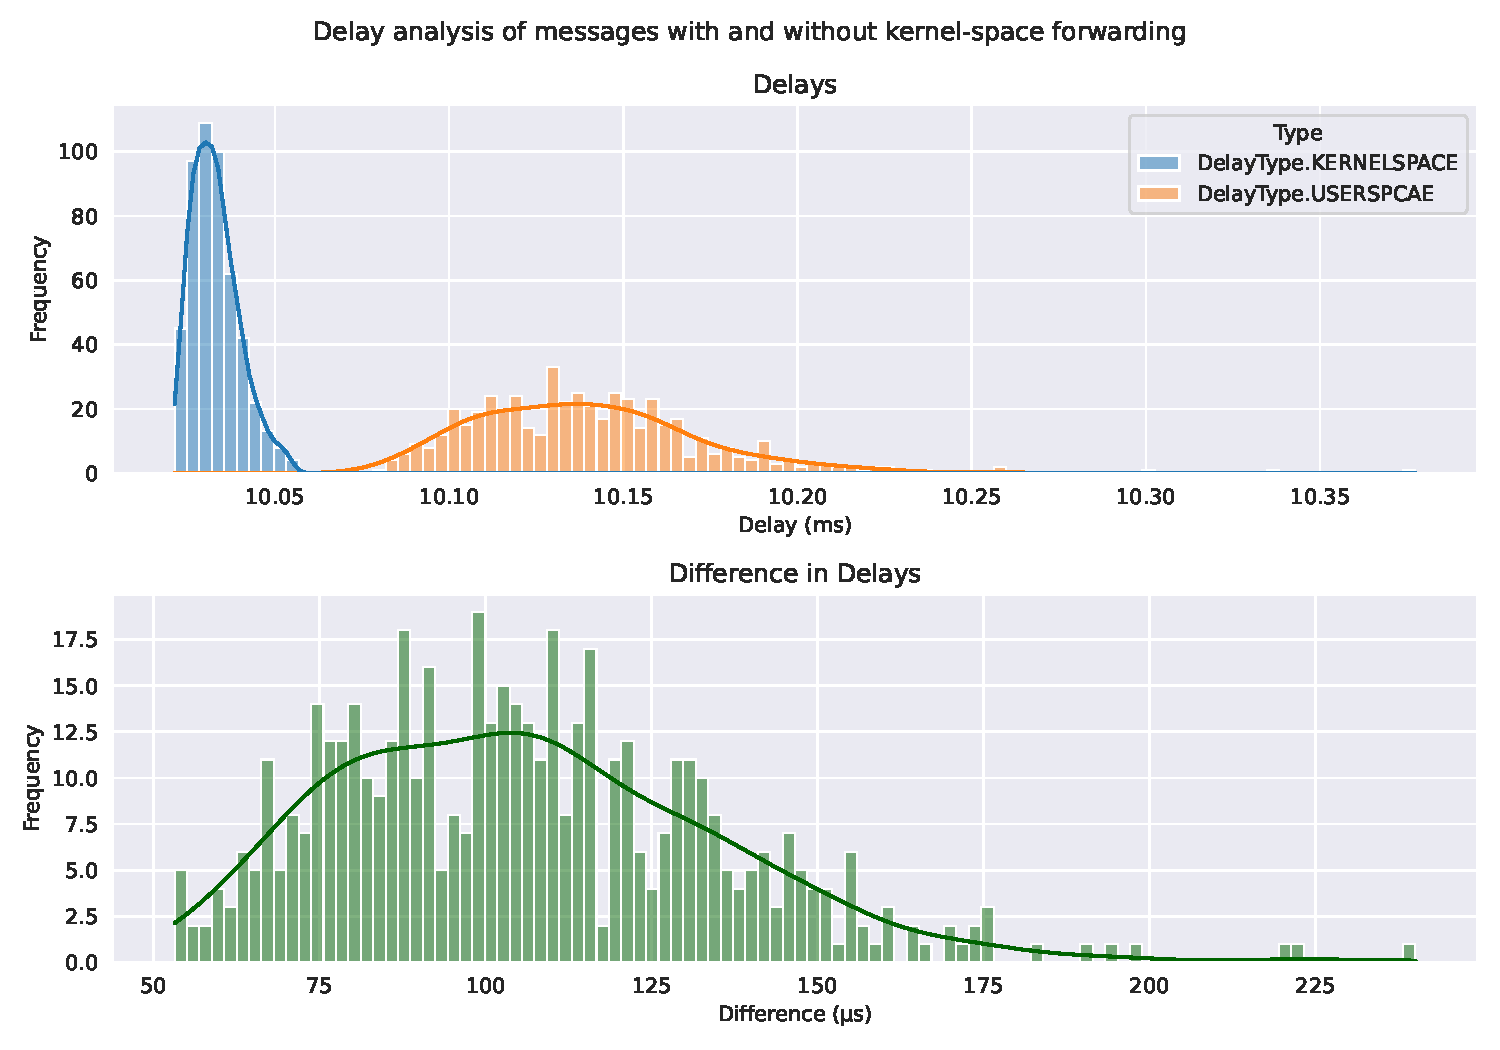
\includegraphics[width=\textwidth]{figures/04_testing_and_results/delays_small_packets_simple_userspace.pdf}
    \caption[Delay analysis of eBPF approach]{The blue and orange parts of the plot show the delay of a 
    kernel- and userspace-forwarded packet, respectively. Delay is measured as time passed between
    leaving the server eBPF program and entering the client eBPF program.
    The green part shows the raw difference between the delays of the same packet, which was sent via both 
    kernel- and userspace-forwarding.}\label{fig:delay-improvement}
\end{figure}
\vspace{0.5cm}

\subsection{CPU Utilization Comparison}
Besides showing that our approach reduces packet delay, we also measured that the CPU usage is 
not negatively impacted by our streaming system.
\autoref{fig:cpu-utilization-server},~\ref{fig:cpu-utilization-relay} and~\ref{fig:cpu-utilization-client}
show the CPU usage of the server, relay, and client processes, respectively, both with and without eBPF forwarding.
It is observable that none of the utilizations significantly differs between the two setups.
We created these CPU measurements by accumulating the CPU usage of all processes that are related 
to the respective parts of the setup.
The tag \verb|user| identifies the traditional setup where packets go all the way up to userspace while 
\verb|kernel| identifies the setup where packets are forwarded directly from within the kernel.

\begin{figure}[H]
    \begin{minipage}{0.48\textwidth}
        \centering
        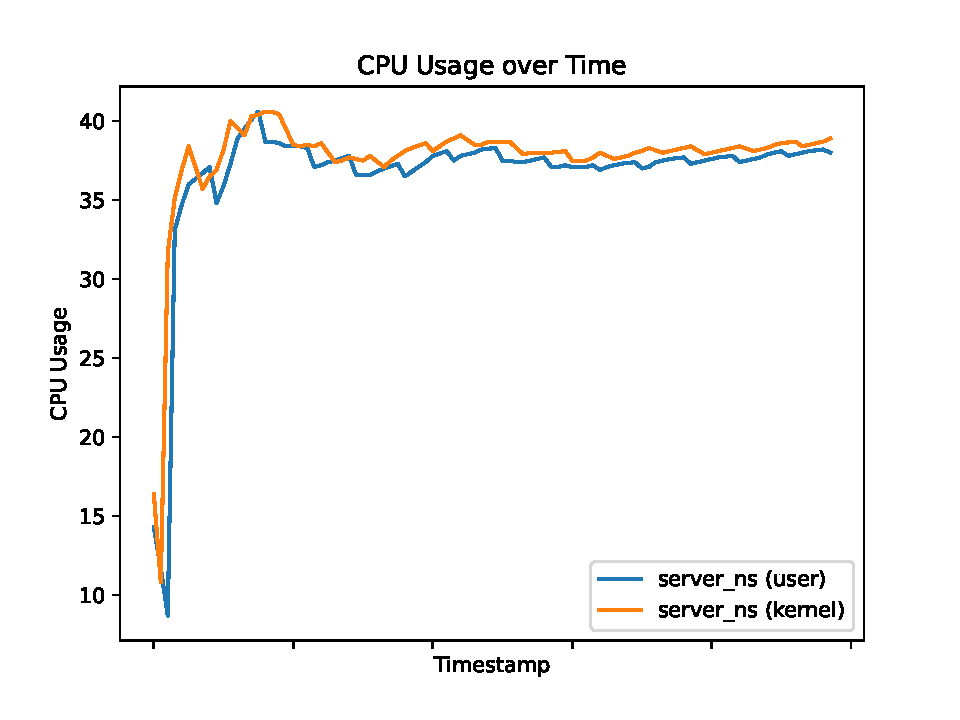
\includegraphics[width=1\linewidth]{figures/04_testing_and_results/cpu_usage_server_ns.pdf}
        \caption[Server CPU usage comparison]{Accumulated server CPU usage comparison.}\label{fig:cpu-utilization-server}
    \end{minipage}\hfill
    \begin{minipage}{0.48\textwidth}
        \centering
        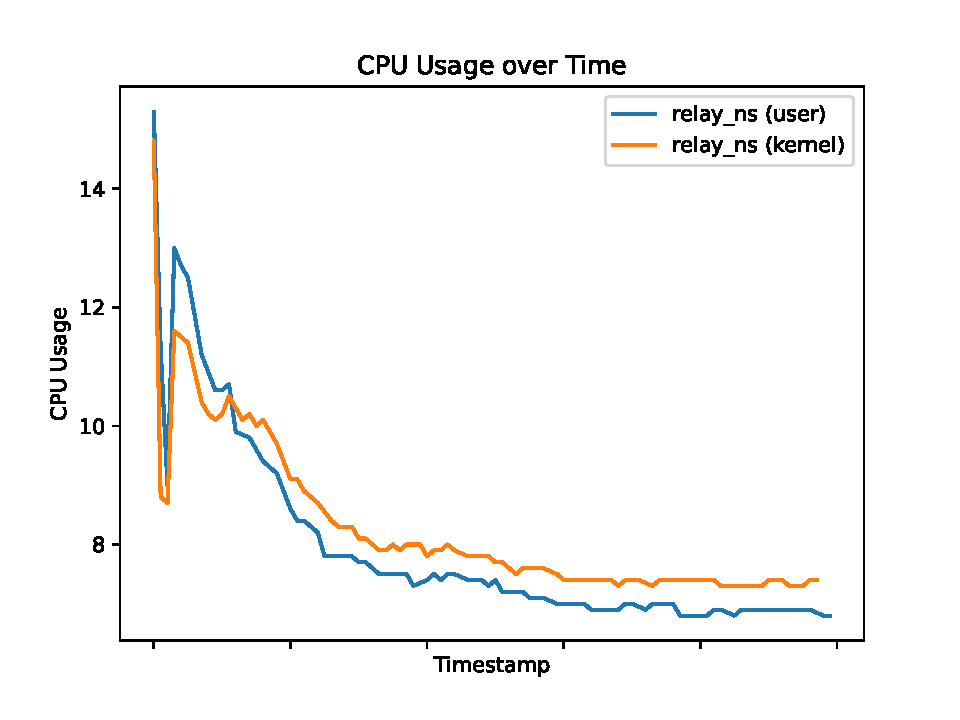
\includegraphics[width=1\linewidth]{figures/04_testing_and_results/cpu_usage_relay_ns.pdf}
        \caption[Relay CPU usage comparison]{Accumulated relay CPU usage comparison.}\label{fig:cpu-utilization-relay}
    \end{minipage}\hfill
    \begin{minipage}{\textwidth}
        \centering
        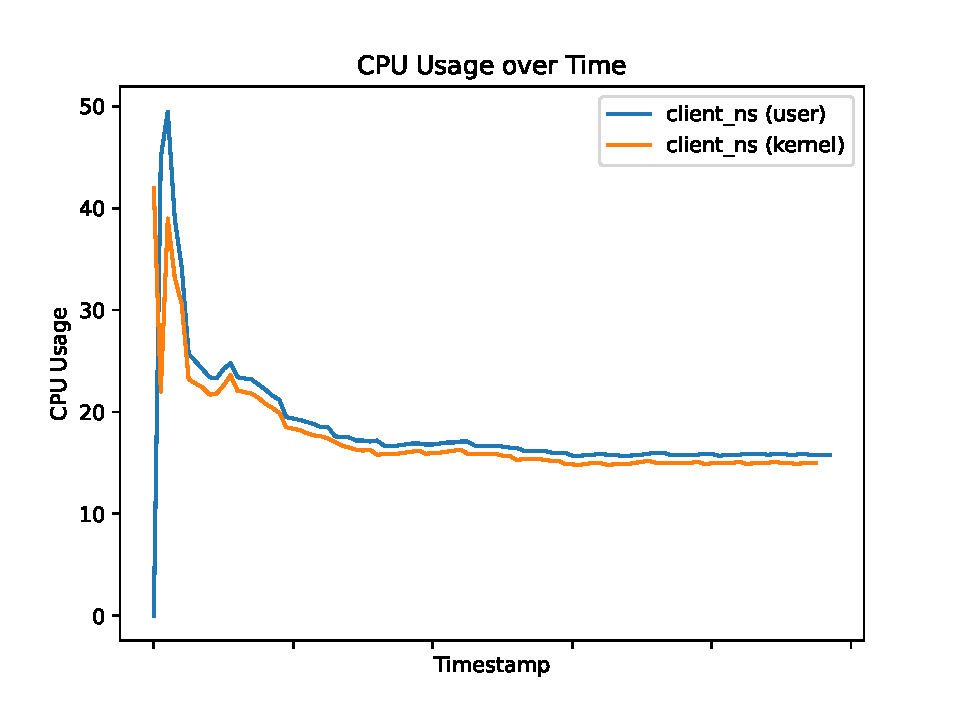
\includegraphics[width=0.48\textwidth]{figures/04_testing_and_results/cpu_usage_client_ns.pdf}
        \caption[Client CPU usage comparison]{Accumulated client CPU usage comparison.}\label{fig:cpu-utilization-client}
    \end{minipage}
\end{figure}

% TODO: remove?
% We also looked more closely which parts of our system take up the most CPU time and compared them
% to the most CPU-intensive parts of the initial userspace forwarding.
% \autoref{tab:cpu-usage-top} shows the top 10 functions that take up the most CPU time in our newly
% developed setup while~\autoref{tab:non-ebpf-cpu-usage-top} shows the same for the old userspace 
% forwarding setup without any eBPF interference. % TODO: make sure reference labels are correct
% We can clearly see that our setup is executing a lot of system calls which is to be expected
% due to the ongoing communication between the userspace and the kernel (i.e.~eBPF maps).
% TODO: measure non ebpf table and compare specific differences 

% \begin{table}
\caption{Table for CPU usage of relay Go processes}
\label{tab:cpu-usage-top}
\begin{tabular}{llllll}
\toprule
flat & flat\% & sum\% & cum & cum\% & cause \\
\midrule
440ms & 28.39\% & 28.39\% & 440ms & 28.39\% & runtime/internal/syscall.Syscall6 \\
140ms & 9.03\% & 37.42\% & 140ms & 9.03\% & runtime.futex \\
120ms & 7.74\% & 45.16\% & 120ms & 7.74\% & runtime.cgocall \\
40ms & 2.58\% & 47.74\% & 40ms & 2.58\% & runtime.write1 \\
30ms & 1.94\% & 49.68\% & 60ms & 3.87\% & runtime.checkTimers \\
30ms & 1.94\% & 51.61\% & 50ms & 3.23\% & runtime.mapaccess2 \\
20ms & 1.29\% & 52.90\% & 70ms & 4.52\% & .../cilium/ebpf/internal/unix.Syscall \\
20ms & 1.29\% & 54.19\% & 20ms & 1.29\% & net.IP.String \\
20ms & 1.29\% & 55.48\% & 20ms & 1.29\% & runtime.casgstatus \\
20ms & 1.29\% & 56.77\% & 20ms & 1.29\% & runtime.duffcopy \\
\bottomrule
\end{tabular}
\end{table}
 % TODO: also include table for "normal" relay and compare difference in what functions use most CPU 
% % \begin{table}
\caption{Table for cumulative CPU usage of relay Go processes}
\label{tab:example}
\begin{tabular}{llllll}
\toprule
flat & flat\% & sum\% & cum & cum\% & cause \\
\midrule
0.44s & 28.39\% & 28.39\% & 0.44s & 28.39\% & runtime/internal/syscall.Syscall6 \\
0 & 0\% & 28.39\% & 0.43s & 27.74\% & runtime.mcall \\
0.01s & 0.65\% & 29.03\% & 0.42s & 27.10\% & runtime.schedule \\
0 & 0\% & 29.03\% & 0.41s & 26.45\% & runtime.park\_m \\
0 & 0\% & 29.03\% & 0.40s & 25.81\% & syscall.RawSyscall6 \\
0.01s & 0.65\% & 29.68\% & 0.32s & 20.65\% & runtime.findRunnable \\
0 & 0\% & 29.68\% & 0.28s & 18.06\% & .../quic-go-prio-packs.(*connection).run \\
0 & 0\% & 29.68\% & 0.28s & 18.06\% & syscall.Syscall \\
0 & 0\% & 29.68\% & 0.23s & 14.84\% & .../quic-go-prio-packs.(*Transport).listen \\
0 & 0\% & 29.68\% & 0.23s & 14.84\% & .../quic-go-prio-packs.(*connection).run.func2 \\
\bottomrule
\end{tabular}
\end{table}
 % TODO: this is kinda useless since it only shows the "wrapping" functions. Maybe remove?
% \begin{table}
    \caption{Table for cumulative CPU usage of relay Go processes without fast-relays enabled.}
    \label{tab:non-ebpf-cpu-usage-top}
    \begin{tabular}{llllll}
    \toprule
    flat & flat\% & sum\% & cum & cum\% & cause \\
    \midrule
    TODO & TODO & TODO & TODO & TODO & TODO \\
    \bottomrule
\end{tabular}
\end{table}
     % TODO: actually measure

\hyperref[chap:appendix-fast-relay]{Appendix A} and~\hyperref[chap:appendix-plain-relay]{B} show 
the syscall usage of a 30-second video streaming example considering a setup with and without eBPF 
forwarding, respectively.
We trace this using\textit{strace} while considering the main process as well as all child processes
it creates and interacts with.
When comparing the two tables, one can see that our approach uses significantly fewer system calls.
This is partially due to a reduced need for userspace synchronization, decreasing the number of \verb|futex| syscalls.
Other syscalls like \verb|epoll_pwait| or \verb|nanosleep| are also used significantly less.

The concrete impact of our setup on system calls can be seen at the bottom 
of~\hyperref[chap:appendix-fast-relay]{Appendix A} and~\hyperref[chap:appendix-plain-relay]{B} 
where total syscall counts are shown.
The setup using eBPF forwarding uses 225674 during our example transmission, while the traditional setup 
uses 296132 syscalls.
This means our setup uses roughly 24\% fewer syscalls than the traditional one.
Regarding \verb|futex| calls, our setup uses a little more than 34\% 
fewer than the traditional setup, with 21666 calls instead of 32940.
Even bigger percentage differences can be seen for \verb|nanosleep| calls with a reduction of 
approximately 42\% (14293 instead of 24716) and \verb|epoll_pwait| calls with 
an improvement of around 67\% (11289 instead of 34149).

Another observation we made was that the eBPF setup uses fewer \verb|bpf| syscalls than we would have assumed for 
the amount of traffic that happened in the test.
This might be caused by optimizations happening in the eBPF library used by our Go application.
Such optimizations might include reducing the number of \verb|bpf| syscalls 
by combining multiple map reads into one syscall.
We did, however, not investigate how this underlying library works and how our 
eBPF communication could be optimized further.
\section{Summary}\label{sec:summary_ch4}

We have presented the results of comparing our newly developed 
relay design to a traditional relay system without eBPF usage.
We were able to show that the idea of delaying any non-essential
application-layer processing until after the packet was forwarded
does provide a performance benefit, while utilizing a similar 
amount of CPU resources.
The fact that our system works also shows that eBPF is capable of 
providing basic relay functionality despite possible limitations
due to its verifier.
In the following chapter, we will conclude our work and provide
an outlook on future work that can be done in this area.
\newpage
% !TeX root = ../main.tex
% Add the above to each chapter to make compiling the PDF easier in some editors.

\iffalse
    % Mention initial questions:
    % How can we improve the performance of a relay in a media streaming scenario by using eBPF technology?
    % How can we avoid the need to direct a packet through userspace?
    % How to handle the fact that packets are heavily encrypted?
    % What communication between userspace and eBPF program is necessary to keep coherency?
    % How can our approach be generalized to other protocols?
\fi

\chapter{Conclusion}\label{chap:conclusion}

Closing this thesis, in this chapter, we will summarize and conclude our findings 
and give a brief outlook on what one could do to advance the work we have done.
Many of the initial questions we posed in the introduction have been answered
but some areas, even though briefly touched upon, will benefit from further research.

\section{Conclusion}\label{sec:conclusion}
In this thesis, we have shown how one can improve the performance of a relay in a media streaming scenario 
by using eBPF technology.
We explained needed high-level concepts and provided insights into implementation details of a prototype 
showing the feasibility of our approach.
Concluding, we can say that leveraging the high-performance capabilities of eBPF programs and forfeiting 
some universality of a relay design can lead to faster and more deterministic packet processing with 
a similar CPU load.
We thereby answered the initial research questions regarding the possibility of a performance improvement 
and the avoidance of userspace processing.
Our prototype showed the needed communication between the userspace and the eBPF program to keep coherency and, by doing so, answered another research subquestion regarding the necessary communication.
Lastly, throughout our work, we also hinted on how to expand our setup to support other protocols and standards, 
covering the last of our initial questions regarding generalization.

\section{Future Work}\label{sec:future_work}

Here we will mention some parts that still require additional work 
to be done.
The areas that will be mentioned will provide a good starting point
in case one wants to build upon or extend our work.

\subsection{Hardware Offload}
This thesis heavily relies on the fact that the relay can
access certain fields (e.g.~packet-numbers) of the packet, 
which are generally not accessible without prior decryption.
In the current setup, this is made possible by turning off 
encryption altogether but to be of any use in a real-world
scenario, the encryption of incoming and the decryption of
outgoing packets would need to be pushed down below the lowest 
used BPF hook point in the stack.

Future work could focus on developing a hardware offload 
setup similar to those already available for TCP/IP checksum 
offloading~\parencite{tcp-ip-offload-engine}.
We looked for possible smartNICs and libraries that would allow us
to offload en- and decryption.
However, at the time of writing, we could not come up with any viable solution
that works with our current setup. 
We believe one could possibly even put the eBPF program itself on the smartNIC as 
another approach suggests~\parencite{ebpf-offload-smartnics}.
The cited work does consider eBPF/XDP offloading, so further 
research would be required to see if this could be adapted to eBPF/TC 
programs as well.

Despite the current lack of options, previous work in this direction has already been 
done since at least 2019~\parencite{quic-nic-offload}, which makes us hopeful that
integrating smartNIC support into our prototype can be achieved in the near future.

\subsection{Compatibility Expansion}\label{sec:compatibility_expansion}
This thesis used the QUIC protocol together with media over QUIC (MoQ)
to demonstrate how fast-relays, which circumvent userspace by utilizing eBPF programs, can be designed.
However, generally speaking, the design of fast-relays is not limited to
any of these protocols and could be expanded, given modifications to 
necessary fields are possible (i.e.~not prevented by encryption), and
there is a way to accommodate the priority of a packet in the packet itself.
The latter point could always be realized by using part of the payload
which forces a deeper packet inspection within the BPF program but 
avoids the need to fit the priority into the header of an existing 
protocol.

Expanding our approach to other protocols could be interesting for 
many areas outside of media streaming, examples being gaming, 
telesurgery or financial services where a delay-decrease of 
microseconds could help make a system more deterministic and 
thus more reliable.

\subsection{Prototype Completion}\label{sec:prototype_completion}
As mentioned already during the setup description, our prototype 
does leave out some parts of the proposed design.
Despite them not being essential for our proof of concept,
both in functionality and performance, they are still important
for a final product that is intended to be used in a real-world
scenario.

Future work could focus on finalizing the prototype by researching 
and implementing best practices for the areas of congestion handling
and retransmission management, among others.


\appendix{}

\microtypesetup{protrusion=false}
\listoffigures{}
\listoftables{}
\chapter*{Abbreviations}
TODO
\microtypesetup{protrusion=true}
\printbibliography{}
% !TeX root = ../main.tex
% Add the above to each chapter to make compiling the PDF easier in some editors.

% !TeX root = ../main.tex
% Add the above to each chapter to make compiling the PDF easier in some editors.

{\let\clearpage\relax \chapter*{Syscalls with eBPF Forwarding}\label{chap:appendix-fast-relay}
\markboth{Appendix A}{Syscalls with eBPF Forwarding}
\addcontentsline{toc}{chapter}{Appendix A}}
\begin{myverbatim}
% time     seconds  usecs/call     calls    errors syscall
------ ----------- ----------- --------- --------- ------------------
 59,95   17,114866         789     21666      1663 futex
 11,06    3,156126       52602        60           wait4
  7,58    2,163202         151     14293        18 nanosleep
  5,66    1,616939         143     11289         6 epoll_pwait
  3,53    1,006913          33     30236       107 read
  3,28    0,937777          29     32194           fcntl
  1,56    0,444417          22     19860      1005 newfstatat
  1,32    0,376735          33     11354       253 openat
  1,02    0,289889          25     11417           close
  0,90    0,256689          46      5580      5239 epoll_ctl
  0,81    0,230937        4528        51         5 waitid
  0,37    0,104574          21      4898      1812 recvmmsg
  0,36    0,103789          52      1990           sched_yield
  0,32    0,090941           2     32329           lseek
  0,28    0,081038         413       196           clone
  0,25    0,072563          62      1160           getpid
  0,25    0,072532          64      1133           sendmsg
  0,18    0,051164          37      1381        40 rt_sigreturn
  0,18    0,050788         276       184           copy_file_range
  0,17    0,049578          13      3697           getrandom
  0,15    0,043913          39      1114           tgkill
  0,12    0,035065          56       622           fstat
  0,12    0,033083          79       416           getdents64
  0,11    0,031193          14      2178           mmap
  0,06    0,018254          13      1314        22 bpf
  0,05    0,015350          17       875           pread64
  0,05    0,012890        1171        11           restart_syscall
  0,04    0,011800          15       782           rt_sigprocmask
  0,04    0,011269          54       206        12 unlinkat
  0,03    0,009583           7      1262           write
  0,03    0,009384          32       285           madvise
  0,03    0,007470           3      2481      2456 readlink
  0,02    0,007114          48       146           pipe2
  0,02    0,005518          45       120           flock
  0,02    0,005466          14       388           sigaltstack
  0,01    0,004037          11       344           gettid
  0,01    0,002415          34        71           munmap
\end{myverbatim}
\newpage
\begin{myverbatim}
  0,01    0,002413           0      6121           rt_sigaction
  0,01    0,002120           5       354           mprotect
  0,00    0,001381           3       394           brk
  0,00    0,001333          19        70         9 execve
  0,00    0,001316          94        14           clone3
  0,00    0,000767          36        21           unlink
  0,00    0,000614           2       252       153 access
  0,00    0,000448          32        14           vfork
  0,00    0,000276           6        46           rseq
  0,00    0,000258           8        30           getrlimit
  0,00    0,000206           4        46           set_robust_list
  0,00    0,000165           1        87        87 ioctl
  0,00    0,000154           2        76           setrlimit
  0,00    0,000145           2        50           getcwd
  0,00    0,000140          46         3           ftruncate
  0,00    0,000135          10        13           timer_settime
  0,00    0,000132           1        67           prlimit64
  0,00    0,000130          10        13           timer_create
  0,00    0,000092          23         4           mkdirat
  0,00    0,000091           3        23           faccessat2
  0,00    0,000077           3        23         2 setsockopt
  0,00    0,000061           4        13           sysinfo
  0,00    0,000059          14         4           epoll_create1
  0,00    0,000058           4        14           getsockopt
  0,00    0,000053           0        93        32 arch_prctl
  0,00    0,000040          40         1           eventfd2
  0,00    0,000036           7         5           socket
  0,00    0,000031          31         1           epoll_wait
  0,00    0,000028           0        32           sched_getaffinity
  0,00    0,000024           0        32           set_tid_address
  0,00    0,000022           5         4           bind
  0,00    0,000017           5         3           timer_delete
  0,00    0,000016           8         2         2 statfs
  0,00    0,000015           2         7           getrusage
  0,00    0,000015           7         2           fallocate
  0,00    0,000013           6         2           getsockname
  0,00    0,000009           0       137           dup3
  0,00    0,000007           3         2           setitimer
  0,00    0,000006           1         4           chmod
  0,00    0,000006           6         1           utimensat
  0,00    0,000004           0         8           umask
  0,00    0,000003           1         2           uname
\end{myverbatim}
\newpage
\begin{myverbatim}
  0,00    0,000000           0         1           readlinkat
------ ----------- ----------- --------- --------- ------------------
100,00   28,548177         126    225674     12923 total
\end{myverbatim}
% !TeX root = ../main.tex
% Add the above to each chapter to make compiling the PDF easier in some editors.

{\let\clearpage\relax \chapter*{Syscalls without eBPF Forwarding}
\label{chap:appendix-plain-relay}
\markboth{Appendix B}{Syscalls without eBPF Forwarding}
\addcontentsline{toc}{chapter}{Appendix B}}
\begin{myverbatim}
% time     seconds  usecs/call     calls    errors syscall
------ ----------- ----------- --------- --------- ------------------
 64,71   29,089191         883     32940      3320 futex
  9,53    4,282788      101971        42           wait4
  7,21    3,242993          94     34149        18 epoll_pwait
  6,64    2,982646         120     24716        35 nanosleep
  2,70    1,212353          39     30601        49 read
  2,01    0,901806          28     31863           fcntl
  0,97    0,437349          22     19794      1005 newfstatat
  0,89    0,401939          33     11862           sendmsg
  0,71    0,319470          18     17115           getrandom
  0,68    0,307659          27     11274       253 openat
  0,54    0,243391          21     11215           close
  0,49    0,219378          40      5414      5221 epoll_ctl
  0,46    0,206849        6894        30         2 waitid
  0,38    0,172377          22      7719      2739 recvmmsg
  0,36    0,162222        1763        92           pipe2
  0,29    0,131692          68      1912           getpid
  0,25    0,112894          40      2798           sched_yield
  0,20    0,090007           2     32309           lseek
  0,17    0,075008          39      1884           tgkill
  0,13    0,058566          26      2237       200 rt_sigreturn
  0,10    0,045475         247       184           copy_file_range
  0,09    0,040321         268       150           clone
  0,08    0,034742          83       415           getdents64
  0,06    0,028940          46       622           fstat
  0,06    0,028247          15      1791           mmap
  0,06    0,026298          15      1751           write
  0,03    0,013730          39       349           madvise
  0,03    0,013598         755        18         2 restart_syscall
  0,03    0,012830          15       831           pread64
  0,02    0,010814          52       206        12 unlinkat
  0,02    0,008929          14       612           rt_sigprocmask
  0,02    0,007546           3      2481      2456 readlink
  0,01    0,003969          12       318           sigaltstack
  0,01    0,003938          32       120           flock
  0,01    0,003676           0      4326           rt_sigaction
  0,01    0,003366          59        57           munmap
  0,01    0,003175          11       281           gettid
\end{myverbatim}
\newpage
\begin{myverbatim}
  0,00    0,002230           8       255           mprotect
  0,00    0,001428          27        52         9 execve
  0,00    0,001425           3       362           brk
  0,00    0,001124          80        14           clone3
  0,00    0,000681          29        23           getrlimit
  0,00    0,000510          56         9           timer_delete
  0,00    0,000449          21        21           unlink
  0,00    0,000362           1       241       142 access
  0,00    0,000336           9        35           rseq
  0,00    0,000270          20        13           timer_create
  0,00    0,000223          17        13           timer_settime
  0,00    0,000200           5        35           set_robust_list
  0,00    0,000157           3        50           getcwd
  0,00    0,000156          11        14           vfork
  0,00    0,000127           1        87        87 ioctl
  0,00    0,000112           4        23           faccessat2
  0,00    0,000091           3        23         2 setsockopt
  0,00    0,000086           1        51           setrlimit
  0,00    0,000081          16         5           socket
  0,00    0,000079           5        14           getsockopt
  0,00    0,000079          39         2           fallocate
  0,00    0,000066           1        56           prlimit64
  0,00    0,000053          17         3           ftruncate
  0,00    0,000052           4        13           sysinfo
  0,00    0,000051          12         4           bind
  0,00    0,000050          12         4           mkdirat
  0,00    0,000036           0        64        21 arch_prctl
  0,00    0,000035           0        90           dup3
  0,00    0,000031           1        25           sched_getaffinity
  0,00    0,000025           6         4           chmod
  0,00    0,000017           0        21           set_tid_address
  0,00    0,000016           8         2           setitimer
  0,00    0,000016           5         3           epoll_create1
  0,00    0,000015           1         8           umask
  0,00    0,000014           7         2         2 statfs
  0,00    0,000012           1         7           getrusage
  0,00    0,000010           5         2           getsockname
  0,00    0,000009           9         1           utimensat
  0,00    0,000004           2         2           uname
  0,00    0,000000           0         1           readlinkat
------ ----------- ----------- --------- --------- ------------------
100,00   44,950890         151    296132     15575 total
\end{myverbatim}

\end{document}
